\documentclass[10pt]{article}  

%%%%%%%% PREÁMBULO %%%%%%%%%%%%
\title{Plantilla para prácticas de UPIITA}
\usepackage[spanish]{babel} %Indica que escribiermos en español
\usepackage[utf8]{inputenc} %Indica qué codificación se está usando ISO-8859-1(latin1)  o utf8  
\usepackage{amsmath} % Comandos extras para matemáticas (cajas para ecuaciones,
% etc)
\usepackage{amssymb} % Simbolos matematicos (por lo tanto)
\usepackage{graphicx} % Incluir imágenes en LaTeX
\usepackage{color} % Para colorear texto
\usepackage{subfigure} % subfiguras
\usepackage{float} %Podemos usar el especificador [H] en las figuras para que se
% queden donde queramos
\usepackage{capt-of} % Permite usar etiquetas fuera de elementos flotantes
% (etiquetas de figuras)
\usepackage{sidecap} % Para poner el texto de las imágenes al lado
	\sidecaptionvpos{figure}{c} % Para que el texto se alinie al centro vertical
\usepackage{caption} % Para poder quitar numeracion de figuras
\usepackage{commath} % funcionalidades extras para diferenciales, integrales,
% etc (\od, \dif, etc)
\usepackage{cancel} % para cancelar expresiones (\cancelto{0}{x})
 
\usepackage{anysize} 					% Para personalizar el ancho de  los márgenes
\marginsize{2cm}{2cm}{2cm}{2cm} % Izquierda, derecha, arriba, abajo

\usepackage{appendix}
\renewcommand{\appendixname}{Apéndices}
\renewcommand{\appendixtocname}{Apéndices}
\renewcommand{\appendixpagename}{Apéndices} 

% Para que las referencias sean hipervínculos a las figuras o ecuaciones y
% aparezcan en color
\usepackage[colorlinks=true,plainpages=true,citecolor=blue,linkcolor=blue]{hyperref}
%\usepackage{hyperref} 
% Para agregar encabezado y pie de página
\usepackage{fancyhdr} 
\pagestyle{fancy}
\fancyhf{}
\fancyhead[L]{\footnotesize UGR} %encabezado izquierda
\fancyhead[R]{\footnotesize EV}   % dereecha
\fancyfoot[R]{\footnotesize Práctica IV}  % Pie derecha
\fancyfoot[C]{\thepage}  % centro
\fancyfoot[L]{\footnotesize Master en Ingeniería Informática}  %izquierda
\renewcommand{\footrulewidth}{0.4pt}

% Directorio para las imágenes
\graphicspath{{/Users/jesusgarciamanday/Desktop/Master/EV/Practicas/Practica4/p4/Imagenes/}}


\usepackage{listings} % Para usar código fuente
\definecolor{dkgreen}{rgb}{0,0.6,0} % Definimos colores para usar en el código
\definecolor{gray}{rgb}{0.5,0.5,0.5} 
% configuración para el lenguaje que queramos utilizar
\lstset{language=Matlab,
   keywords={break,case,catch,continue,else,elseif,end,for,function,
      global,if,otherwise,persistent,return,switch,try,while},
   basicstyle=\ttfamily,
   keywordstyle=\color{blue},
   commentstyle=\color{red},
   stringstyle=\color{dkgreen},
   numbers=left,
   numberstyle=\tiny\color{gray},
   stepnumber=1,
   numbersep=10pt,
   backgroundcolor=\color{white},
   tabsize=4,
   showspaces=false,
   showstringspaces=false}

\newcommand{\sen}{\operatorname{\sen}}	% Definimos el comando \sen para el seno
%en español

%%%%%%%% TERMINA PREÁMBULO %%%%%%%%%%%%

\begin{document}

%%%%%%%%%%%%%%%%%%%%%%%%%%%%%%%%%% PORTADA %%%%%%%%%%%%%%%%%%%%%%%%%%%%%%%%%%%%%%%%%%%%
																					%%%
\begin{center}																		%%%
\newcommand{\HRule}{\rule{\linewidth}{0.5mm}}									%%%\left
 																					%%%
\begin{minipage}{0.48\textwidth} \begin{flushleft}
%
\includegraphics[scale = 0.63]{Imagenes/logo_upiita}
\end{flushleft}\end{minipage}
\begin{minipage}{0.48\textwidth} \begin{flushright}
%
\includegraphics[scale = 0.35]{Imagenes/IPN}
\end{flushright}\end{minipage}

													 								%%%
\vspace*{0.25cm}								%%%
																					%%%	
\textsc{\huge Universidad de Granada}\\[1.5cm]	

\textsc{\LARGE Master en Ingeniería Informática}\\[1.5cm]													%%%

\textsc{\LARGE Entornos Virtuales}\\[1.5cm]													%%%

\begin{minipage}{0.9\textwidth} 
\begin{center}																					%%%
\textsc{\LARGE Practica IV}
\end{center}
\end{minipage}\\[0.5cm]
%%%
    																				%%%
 			\vspace*{1cm}																		%%%
																					%%%
\HRule \\[0.4cm]																	%%%
{ \huge \bfseries Interacción}\\[0.4cm]	%%%
 																					%%%
\HRule \\[1.5cm]																	%%%
 																				%%%
																					%%%
\begin{minipage}{0.46\textwidth}													%%%
\begin{flushleft} \large															%%%
\emph{Autor:}\\	
 Manuel Jesús García Manday
%%%
			%\vspace*{2cm}	
            													%%%
										 						%%%
\end{flushleft}																		%%%
\end{minipage}		
																%%%
\begin{minipage}{0.52\textwidth}		
\vspace{-0.6cm}											%%%
\begin{flushright} \large															%%%													%%%
\end{flushright}																	%%%
\end{minipage}	
\vspace*{1cm}
%\begin{flushleft}
 	
%\end{flushleft}
%%%
 		\flushleft{\textbf{\Large Master en Ingeniería Informática}	}\\																		%%%
\vspace{2cm} 																				
\begin{center}																					

%{\large \today}																	%%%
 			\end{center}												  						
\end{center}							 											
																					
\newpage																		
%%%%%%%%%%%%%%%%%%%% TERMINA PORTADA %%%%%%%%%%%%%%%%%%%%%%%%%%%%%%%%

\tableofcontents 

\newpage

\section{Objetivo.}
El objetivo de esta práctica es aprender a construir entornos interactivos con Blender.


\section{Desarrollo de la práctica.}
Se ha definido el siguiente escenario tomando como objeto a interaccionar el que se ha ido utilizando durante las anteriores prácticas. \\

\begin{figure}[H]
	\begin{center}
	 		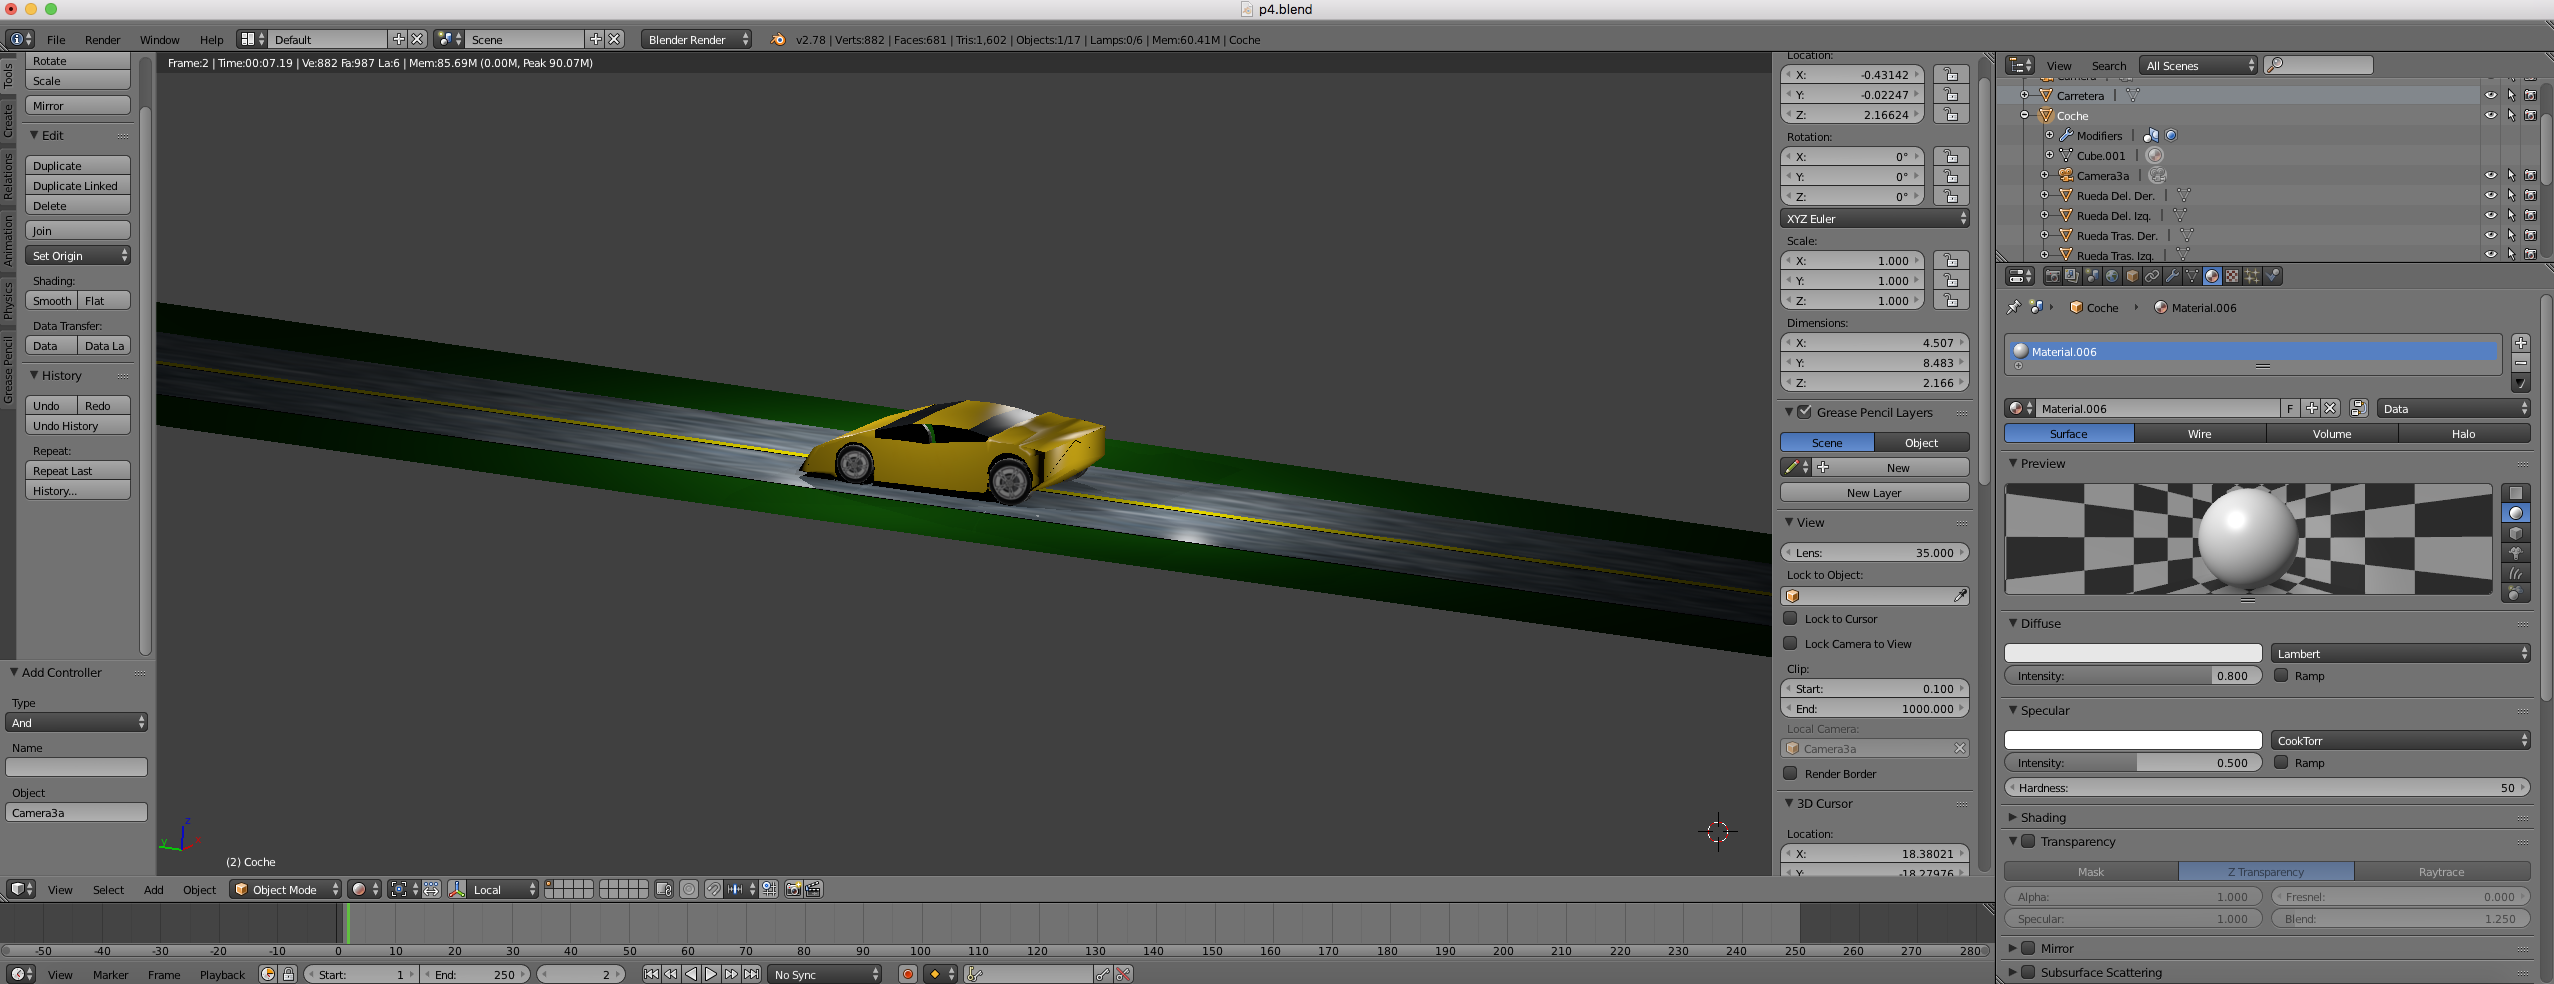
\includegraphics[width = 1.00\textwidth]{Imagenes/p4-img1}
 		\captionof{figure}{\label{fig:IPN}Escenario.} 
	\end{center} 
\end{figure}


\subsection{Movimiento del avatar.}
En el mismo se puede ver el modelo ``Coche'' colocado sobre un plano como modelo de ``Carretera'' por donde dicho objeto se desplazará hacia delante y hacia atrás realizando el movimiento común de un vehículo. La interacción del modelo ``Coche'' se realizará sobre el modelo ``Carretera'' utilizando el motor Blender Game Engine (BGE).  Para ello tenemos que cambiar la opción del motor a utilizar escogiendo el mencionado anteriormente, y también cambiar el diseño de la pantalla que pasaría de estar por defecto a ``Game Logic'' como se muestra en la siguiente imagen. \\

\begin{figure}[H]
	\begin{center}
	 		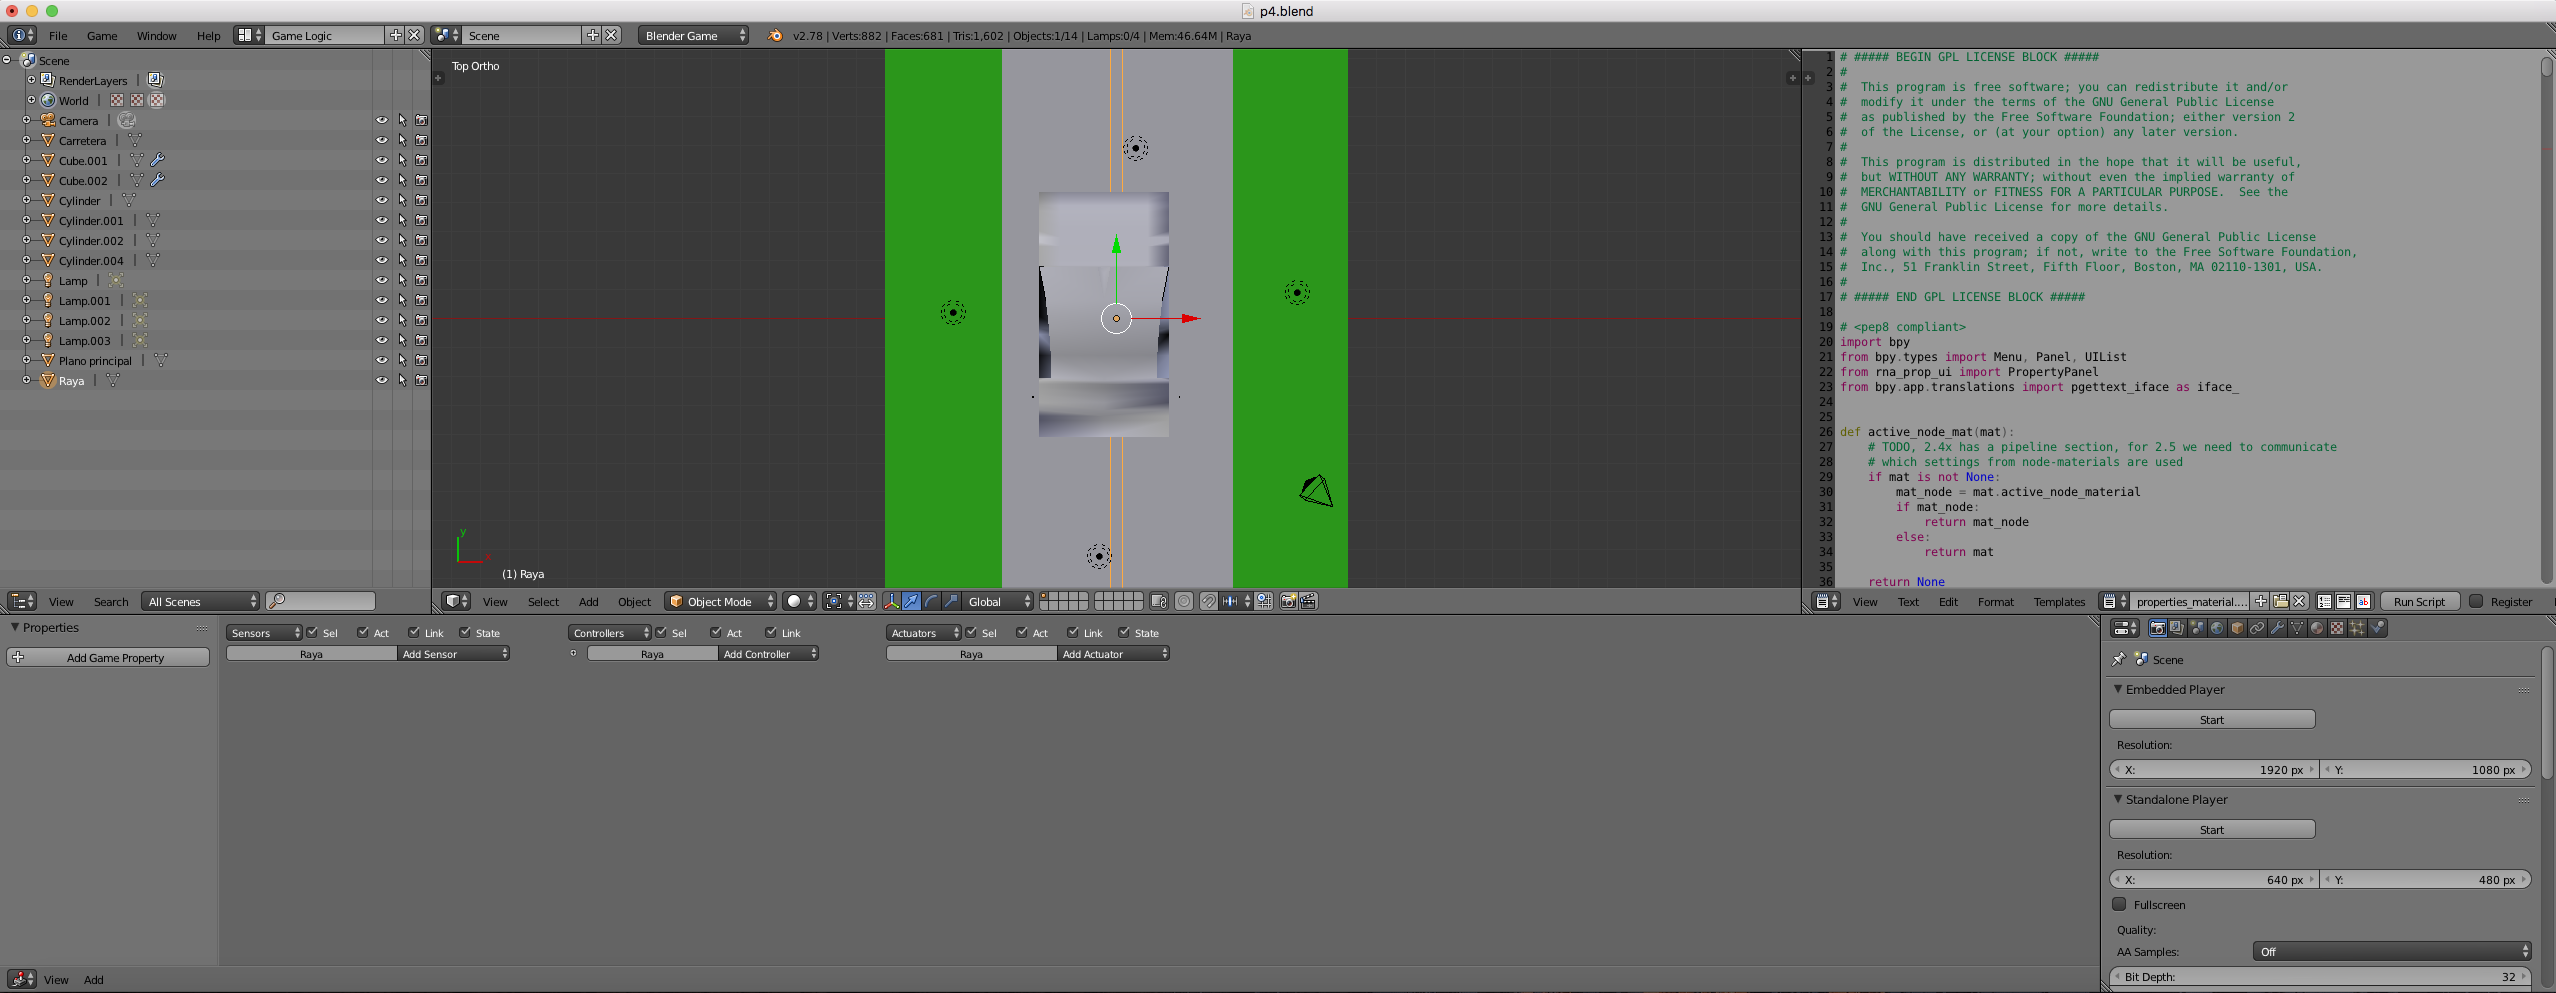
\includegraphics[width = 1.00\textwidth]{Imagenes/p4-img2}
 		\captionof{figure}{\label{fig:IPN}Estableciendo motor y diseño de pantalla.} 
	\end{center} 
\end{figure}

Una vez establecido el motor y el diseño de pantalla y con el modelo del ``Coche'' en modo Objeto, pasamos a configurarle los \textbf{sensores}, \textbf{controladores} y \textbf{actuadores} necesarios para la interacción que va a tener. Le añadiremos un primer sensor de tipo ``Keyboard'' al que le asignaremos la tecla ``W'' para que realice la interacción de desplazarse horizontalmente sobre el objeto ``Carretera''. Este sensor se unirá a un controlador de tipo ``And'' para que cuando se pulse dicha tecla se realice la acción del controlador. El controlador definido será de tipo ``Motion'' lo que hará que el objeto se desplace en función de los parámetros que le indiquemos, en nuestro caso será de 0.50 en el eje Y como se muestra en la siguiente figura. \\

\begin{figure}[H]
	\begin{center}
	 		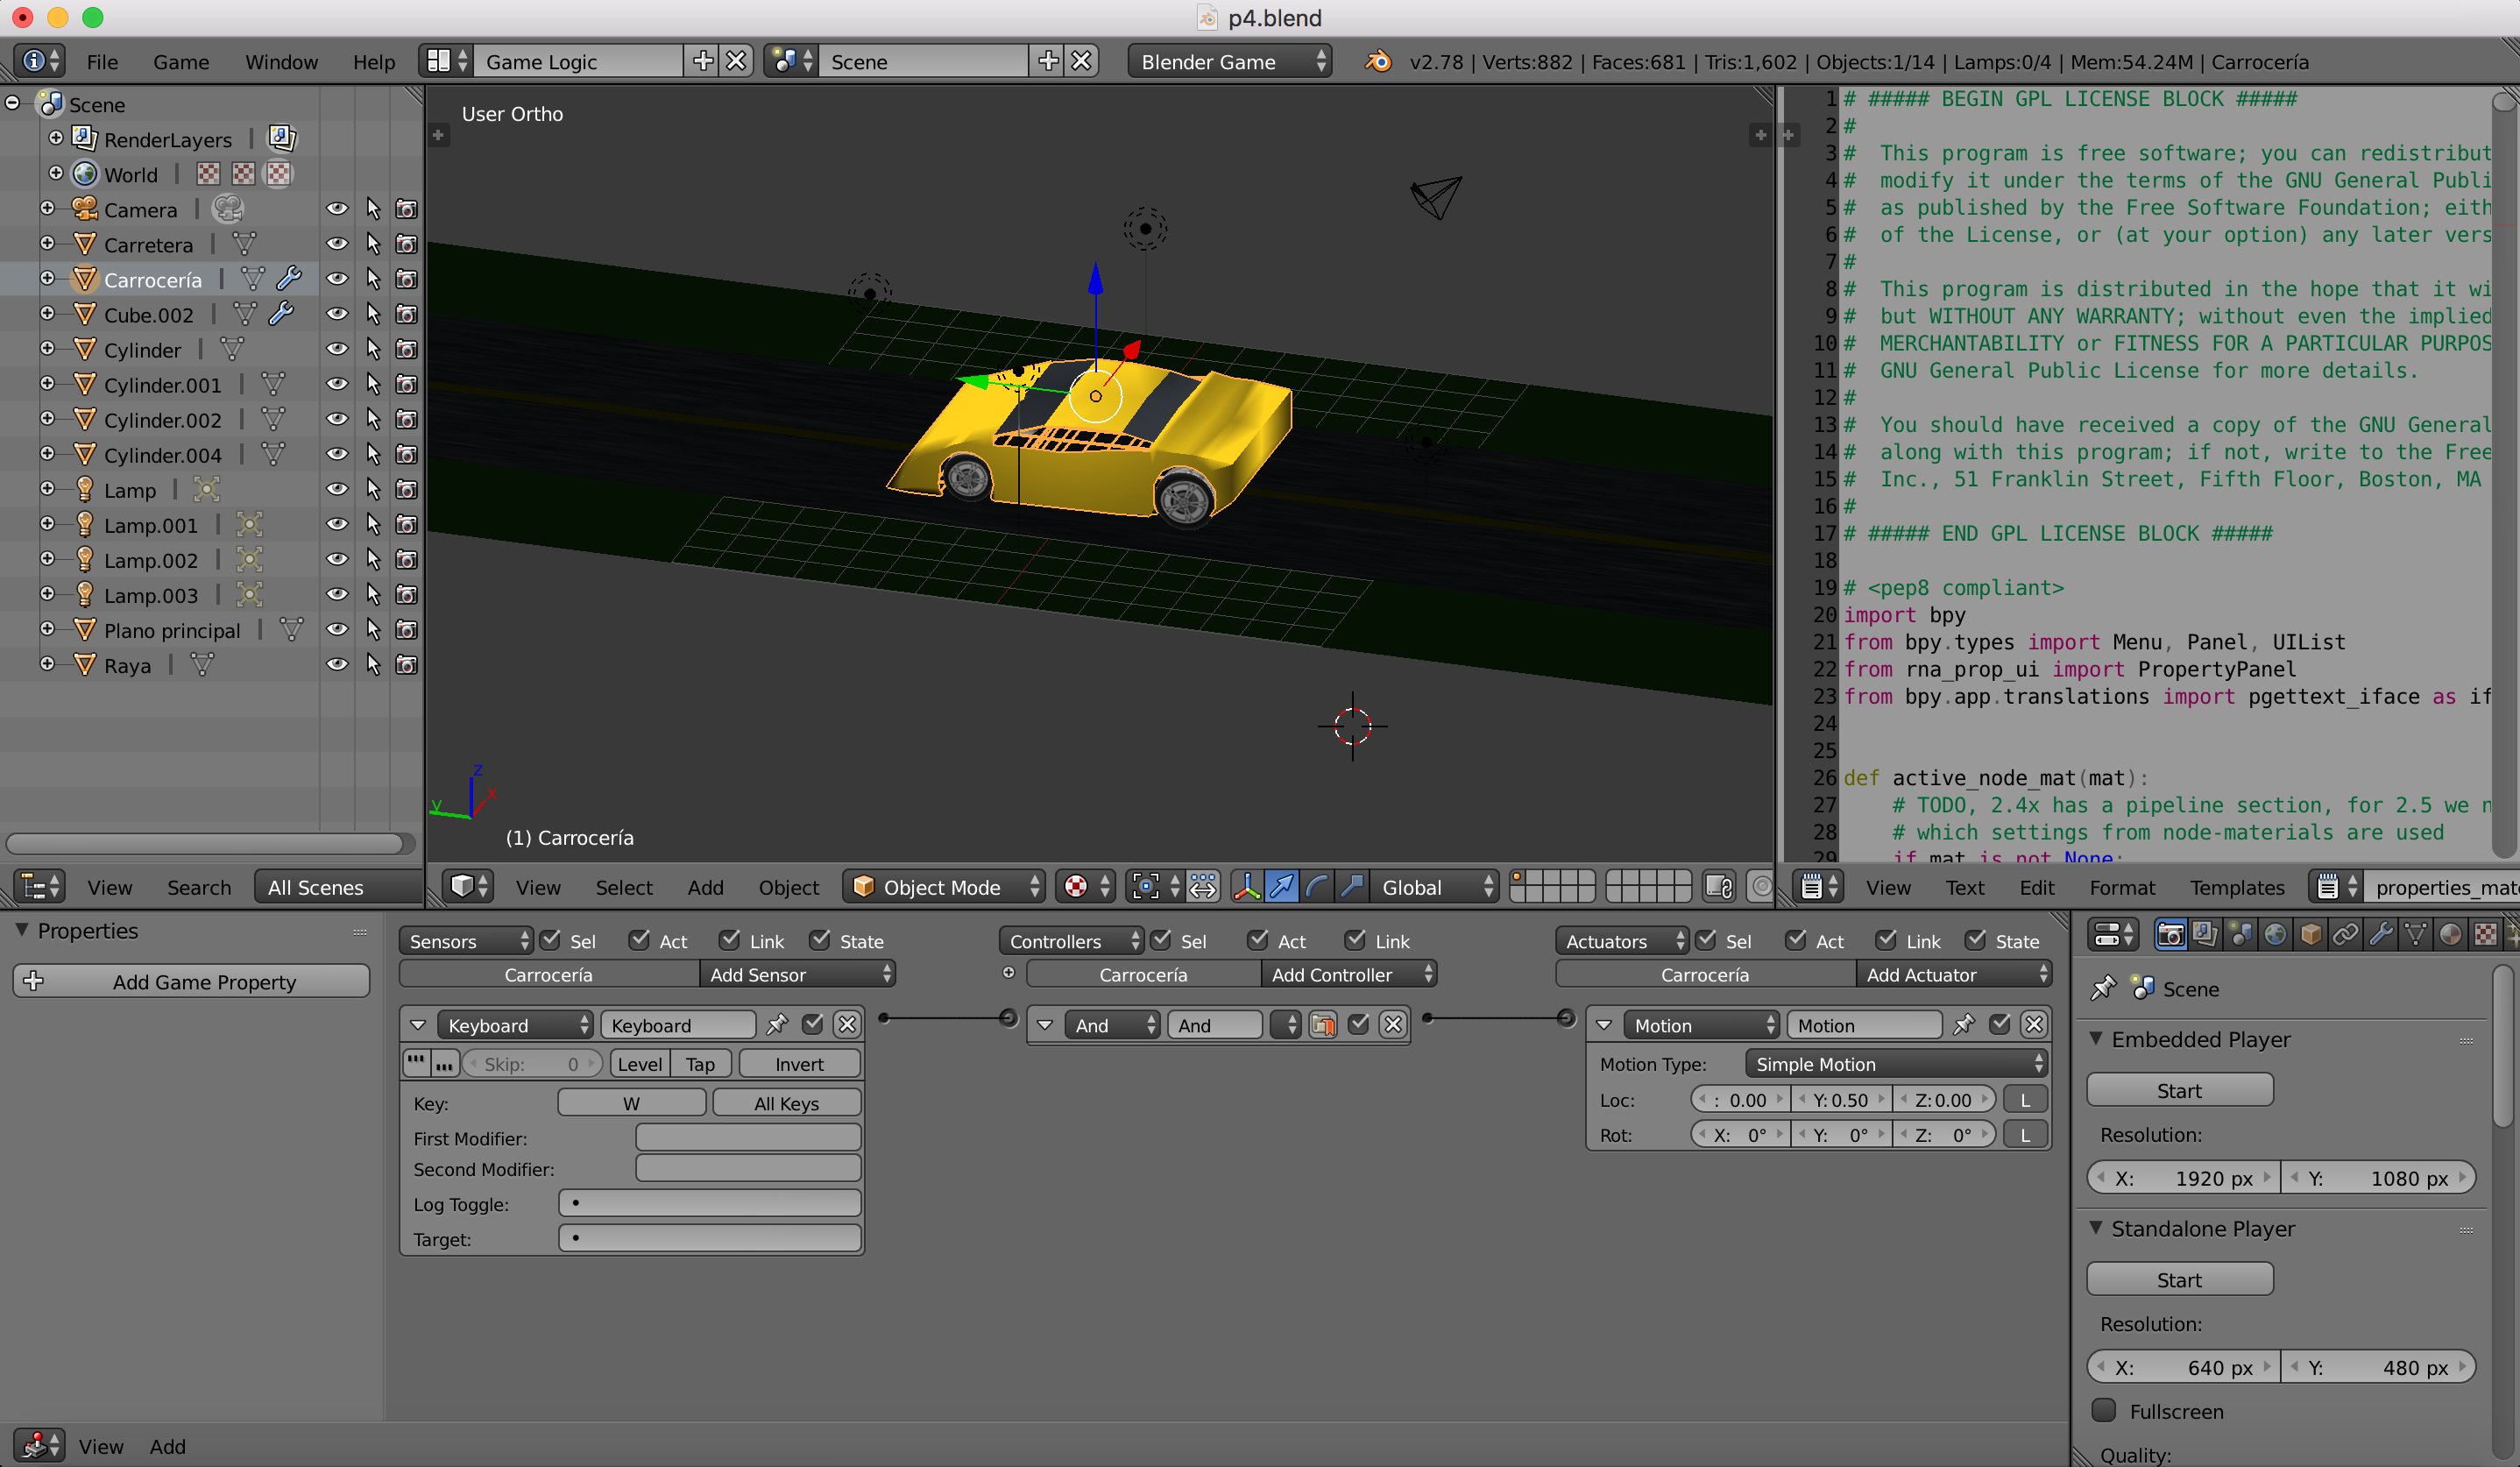
\includegraphics[width = 1.00\textwidth]{Imagenes/p4-img3}
 		\captionof{figure}{\label{fig:IPN}Sensor, controlador y actuador en coche (I).} 
	\end{center} 
\end{figure}

Para el movimiento hacia atrás del coche en la carretera le añadimos otro sensor de tipo ``Keyboard'' y un actuador de tipo ``Motion'' como hicimos en la anterior interacción. La tecla asignada  para realizar el movimiento hacia atrás es la ``S'', mientras que en esta ocasión el parámetro de localización será negativo para que se produzca la interacción que deseamos. Ambos se conectarán por medio de un nuevo controlador de tipo ``And''.\\

\begin{figure}[H]
	\begin{center}
	 		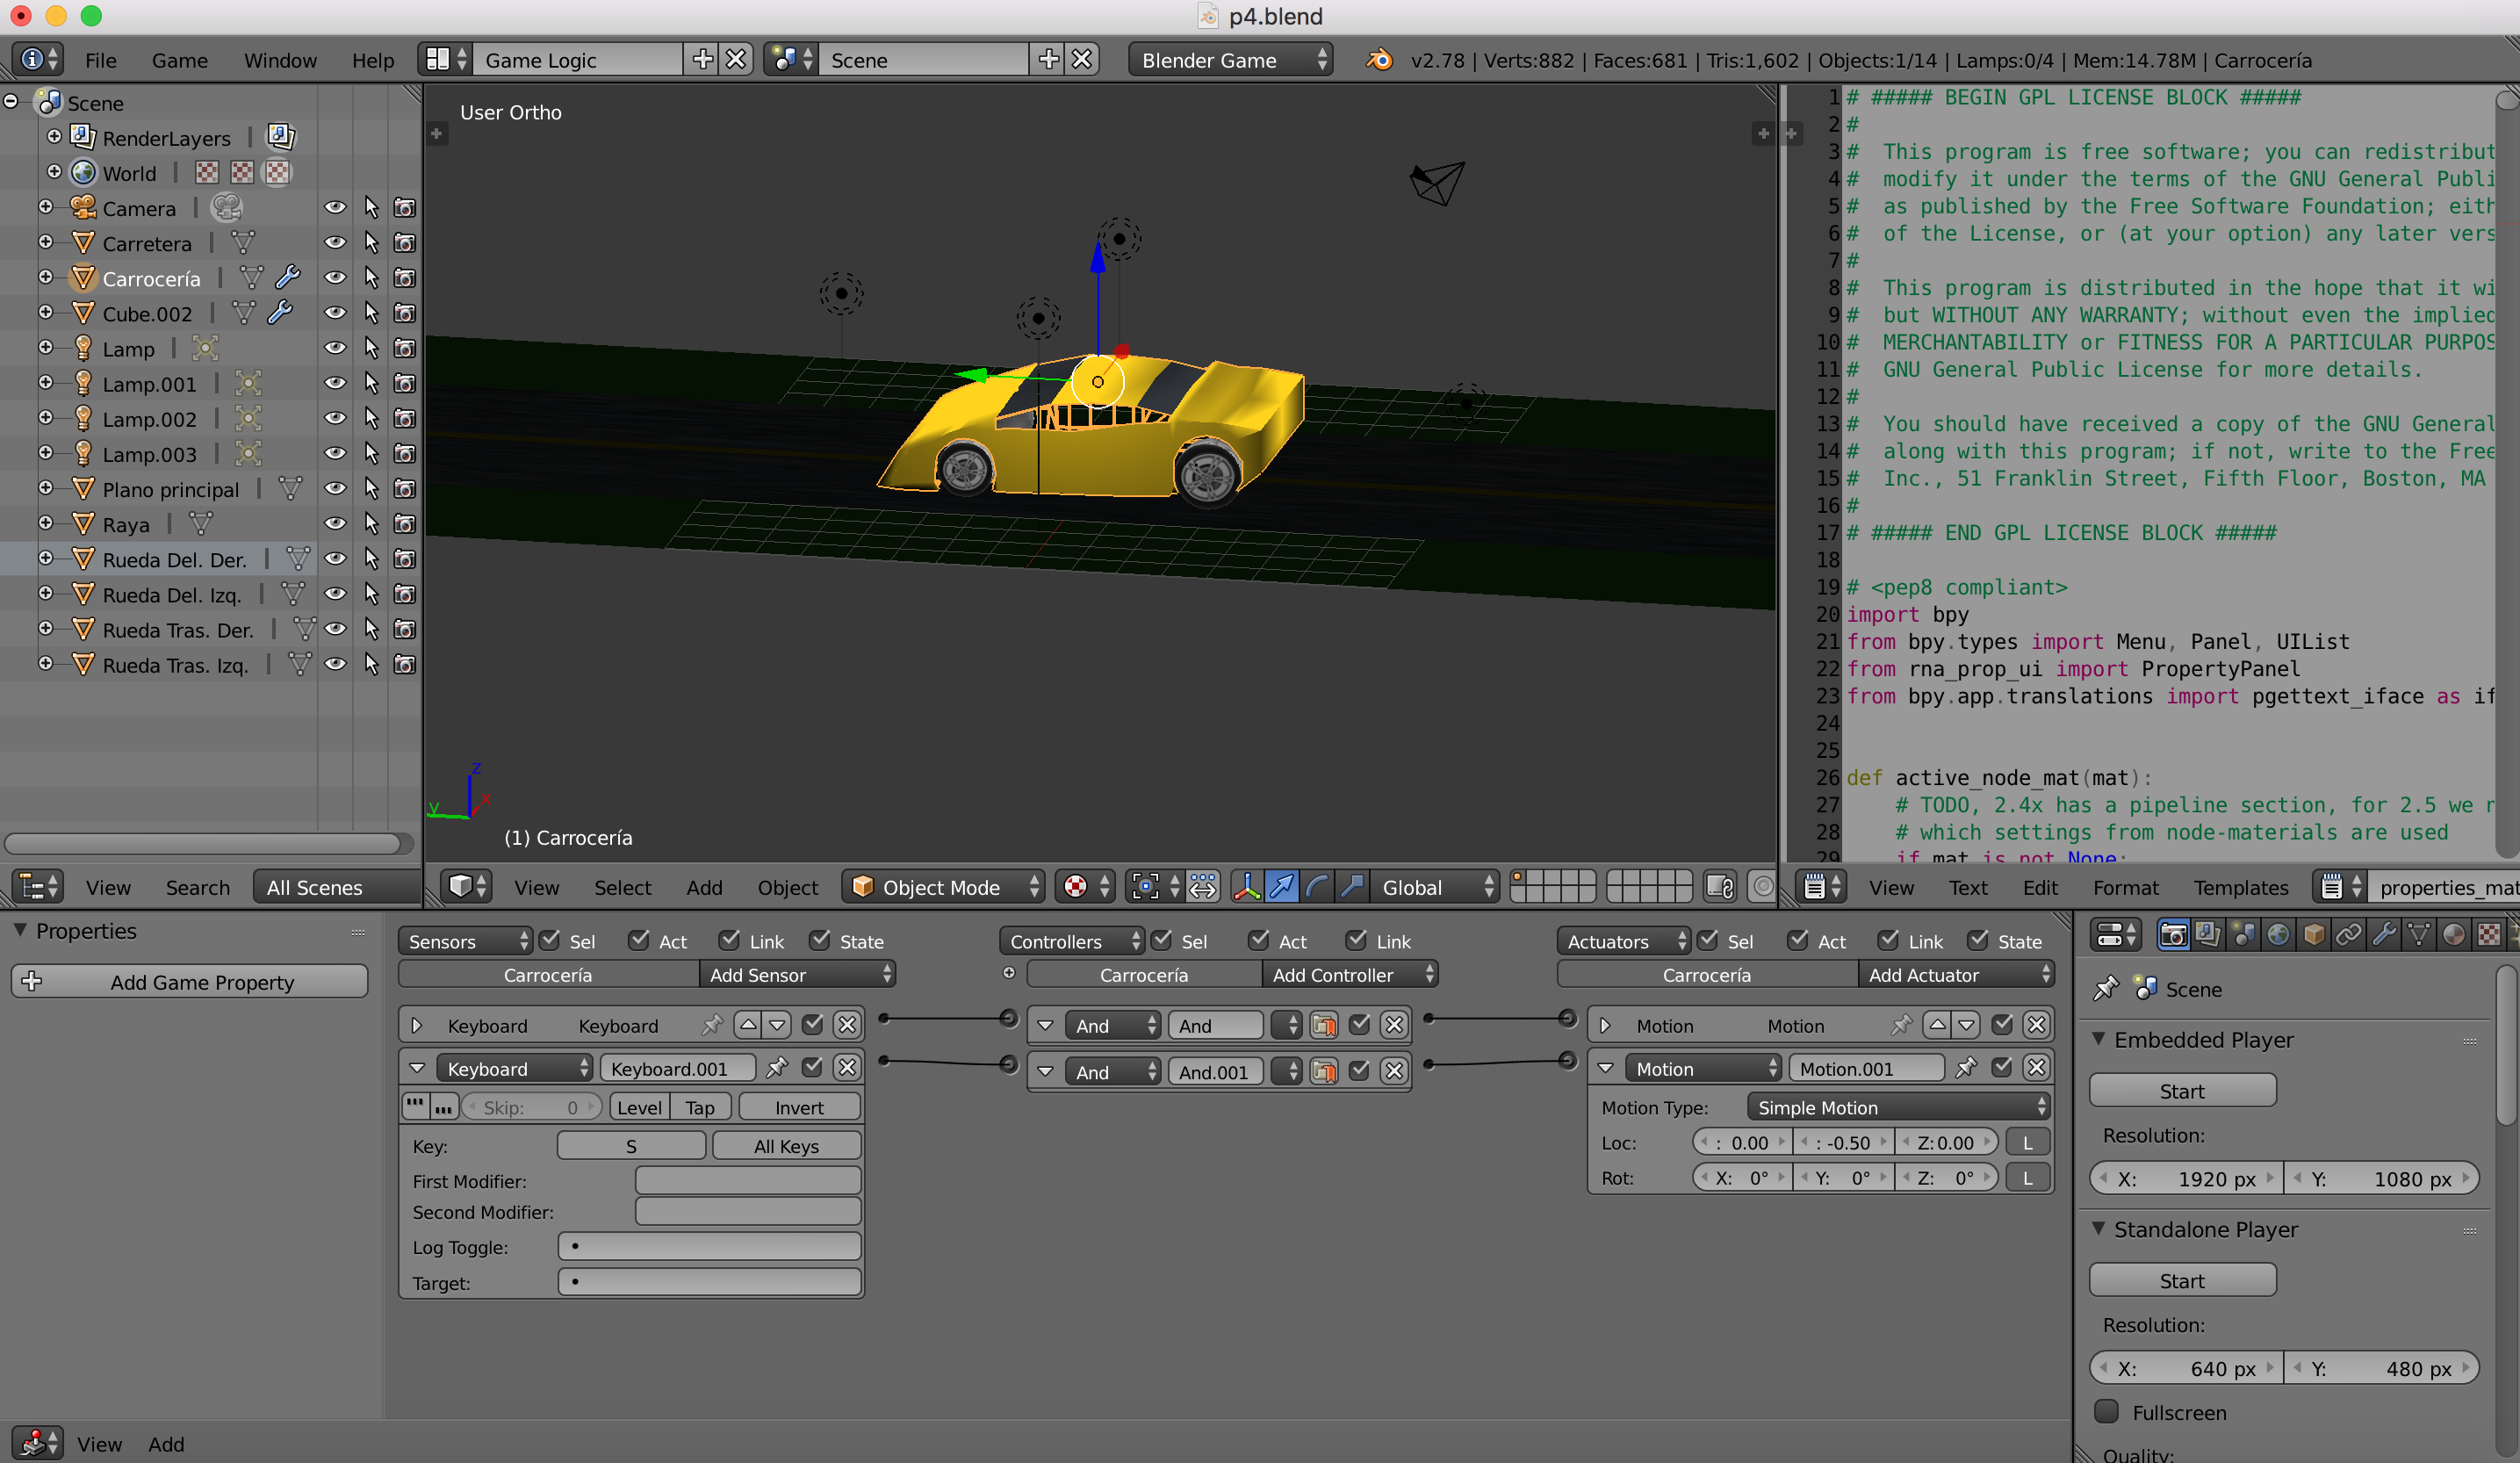
\includegraphics[width = 1.00\textwidth]{Imagenes/p4-img4}
 		\captionof{figure}{\label{fig:IPN}Sensor, controlador y actuador en coche (II).} 
	\end{center} 
\end{figure}

Los siguientes objetos a los que se le van a aplicar interacción son las cuatro ruedas de las que dispone el coche. A dichos objetos se le añadirán los mismos tipos de sensores, controladores y actuadores que para el objeto ``Coche'' pero con diferentes valores de parámetro para que realicen la rotación ligada a los movimientos hacia delante y hacia atrás. Las teclas empleadas serán las mismas, a través de la tecla ``W'' el objeto se deplazará positivamente en el eje Y haciendo que las cuatro ruedas giren en ese mismo sentido, y el mismo efecto aparecerá cuando se pulse la tecla ``S'' pero en este caso el objeto coche se desplazará en el eje negativo Y con el correspondiente giro en ese sentido de las cuatro ruedas que conforman el ``Coche''. \\

El ángulo de giro para ambos casos es el eje Z, siendo 15º cuando el desplazamiento es positivo y -15º cuando es un desplazamiento negativo (sensación de marcha atrás).

\begin{figure}[H]
	\begin{center}
	 		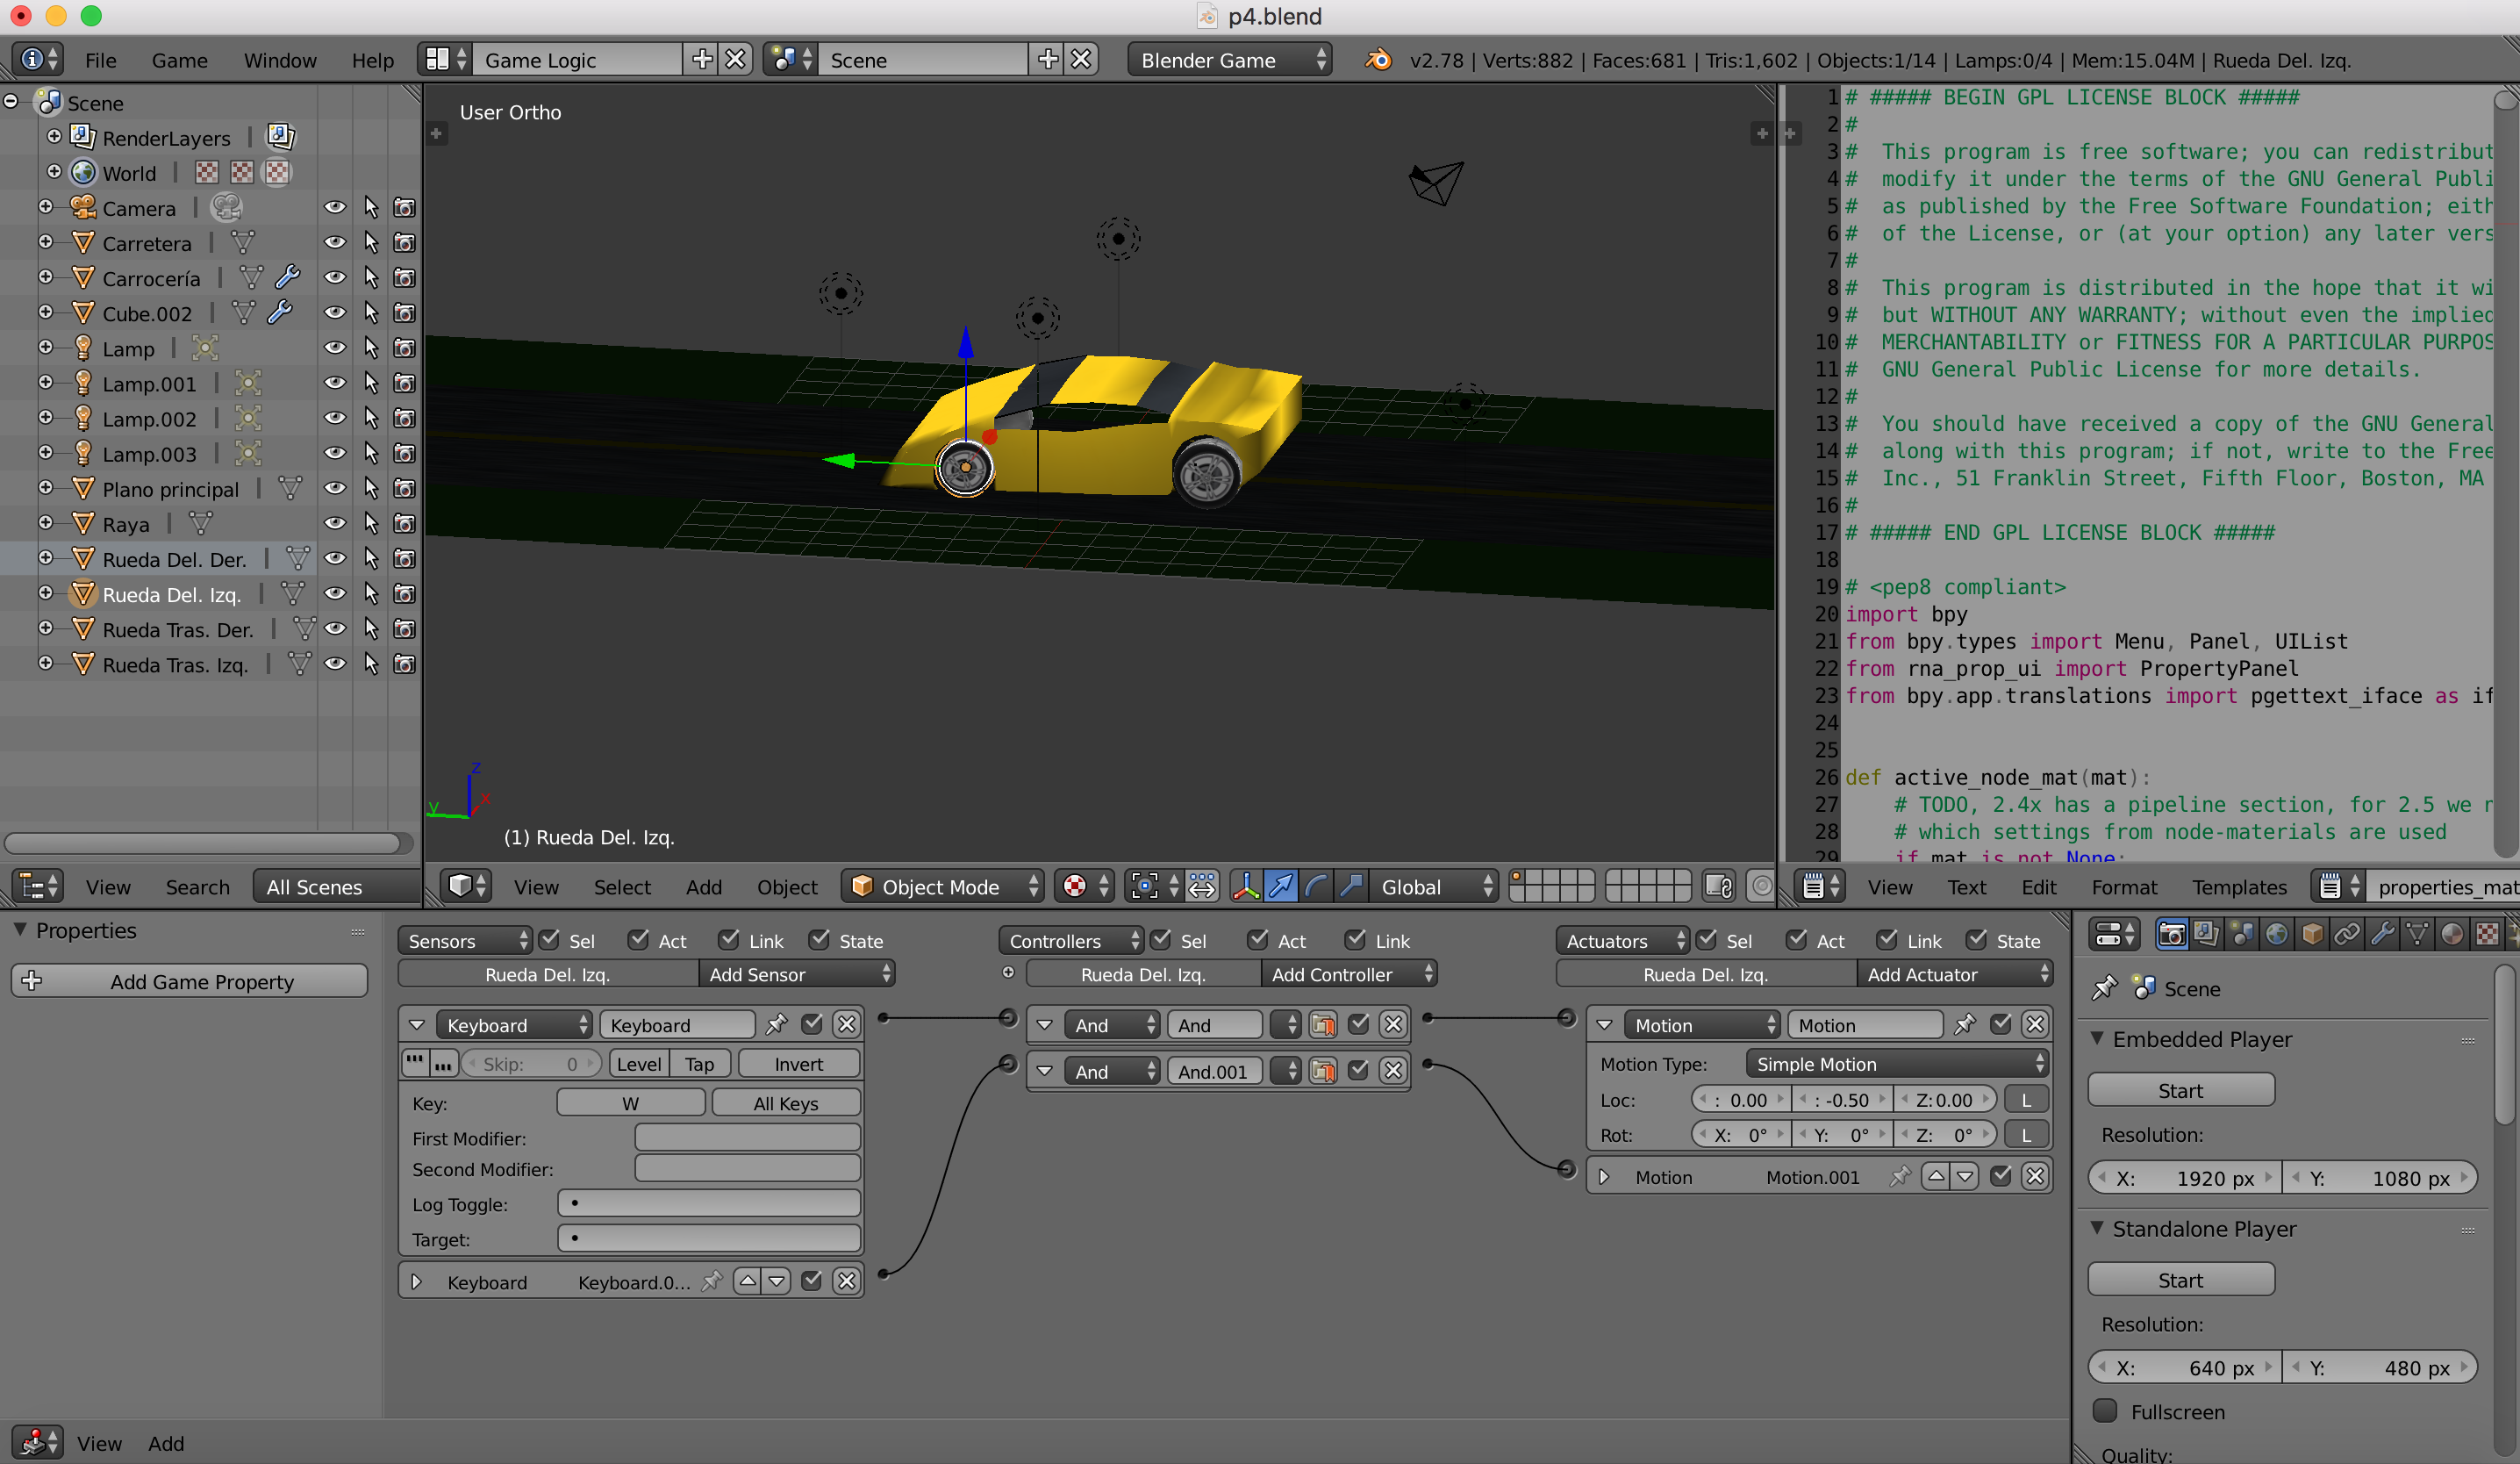
\includegraphics[width = 1.00\textwidth]{Imagenes/p4-img5}
 		\captionof{figure}{\label{fig:IPN}Añadiendo rotación en rueda delantera izquieda (I).} 
	\end{center} 
\end{figure}

\begin{figure}[H]
	\begin{center}
	 		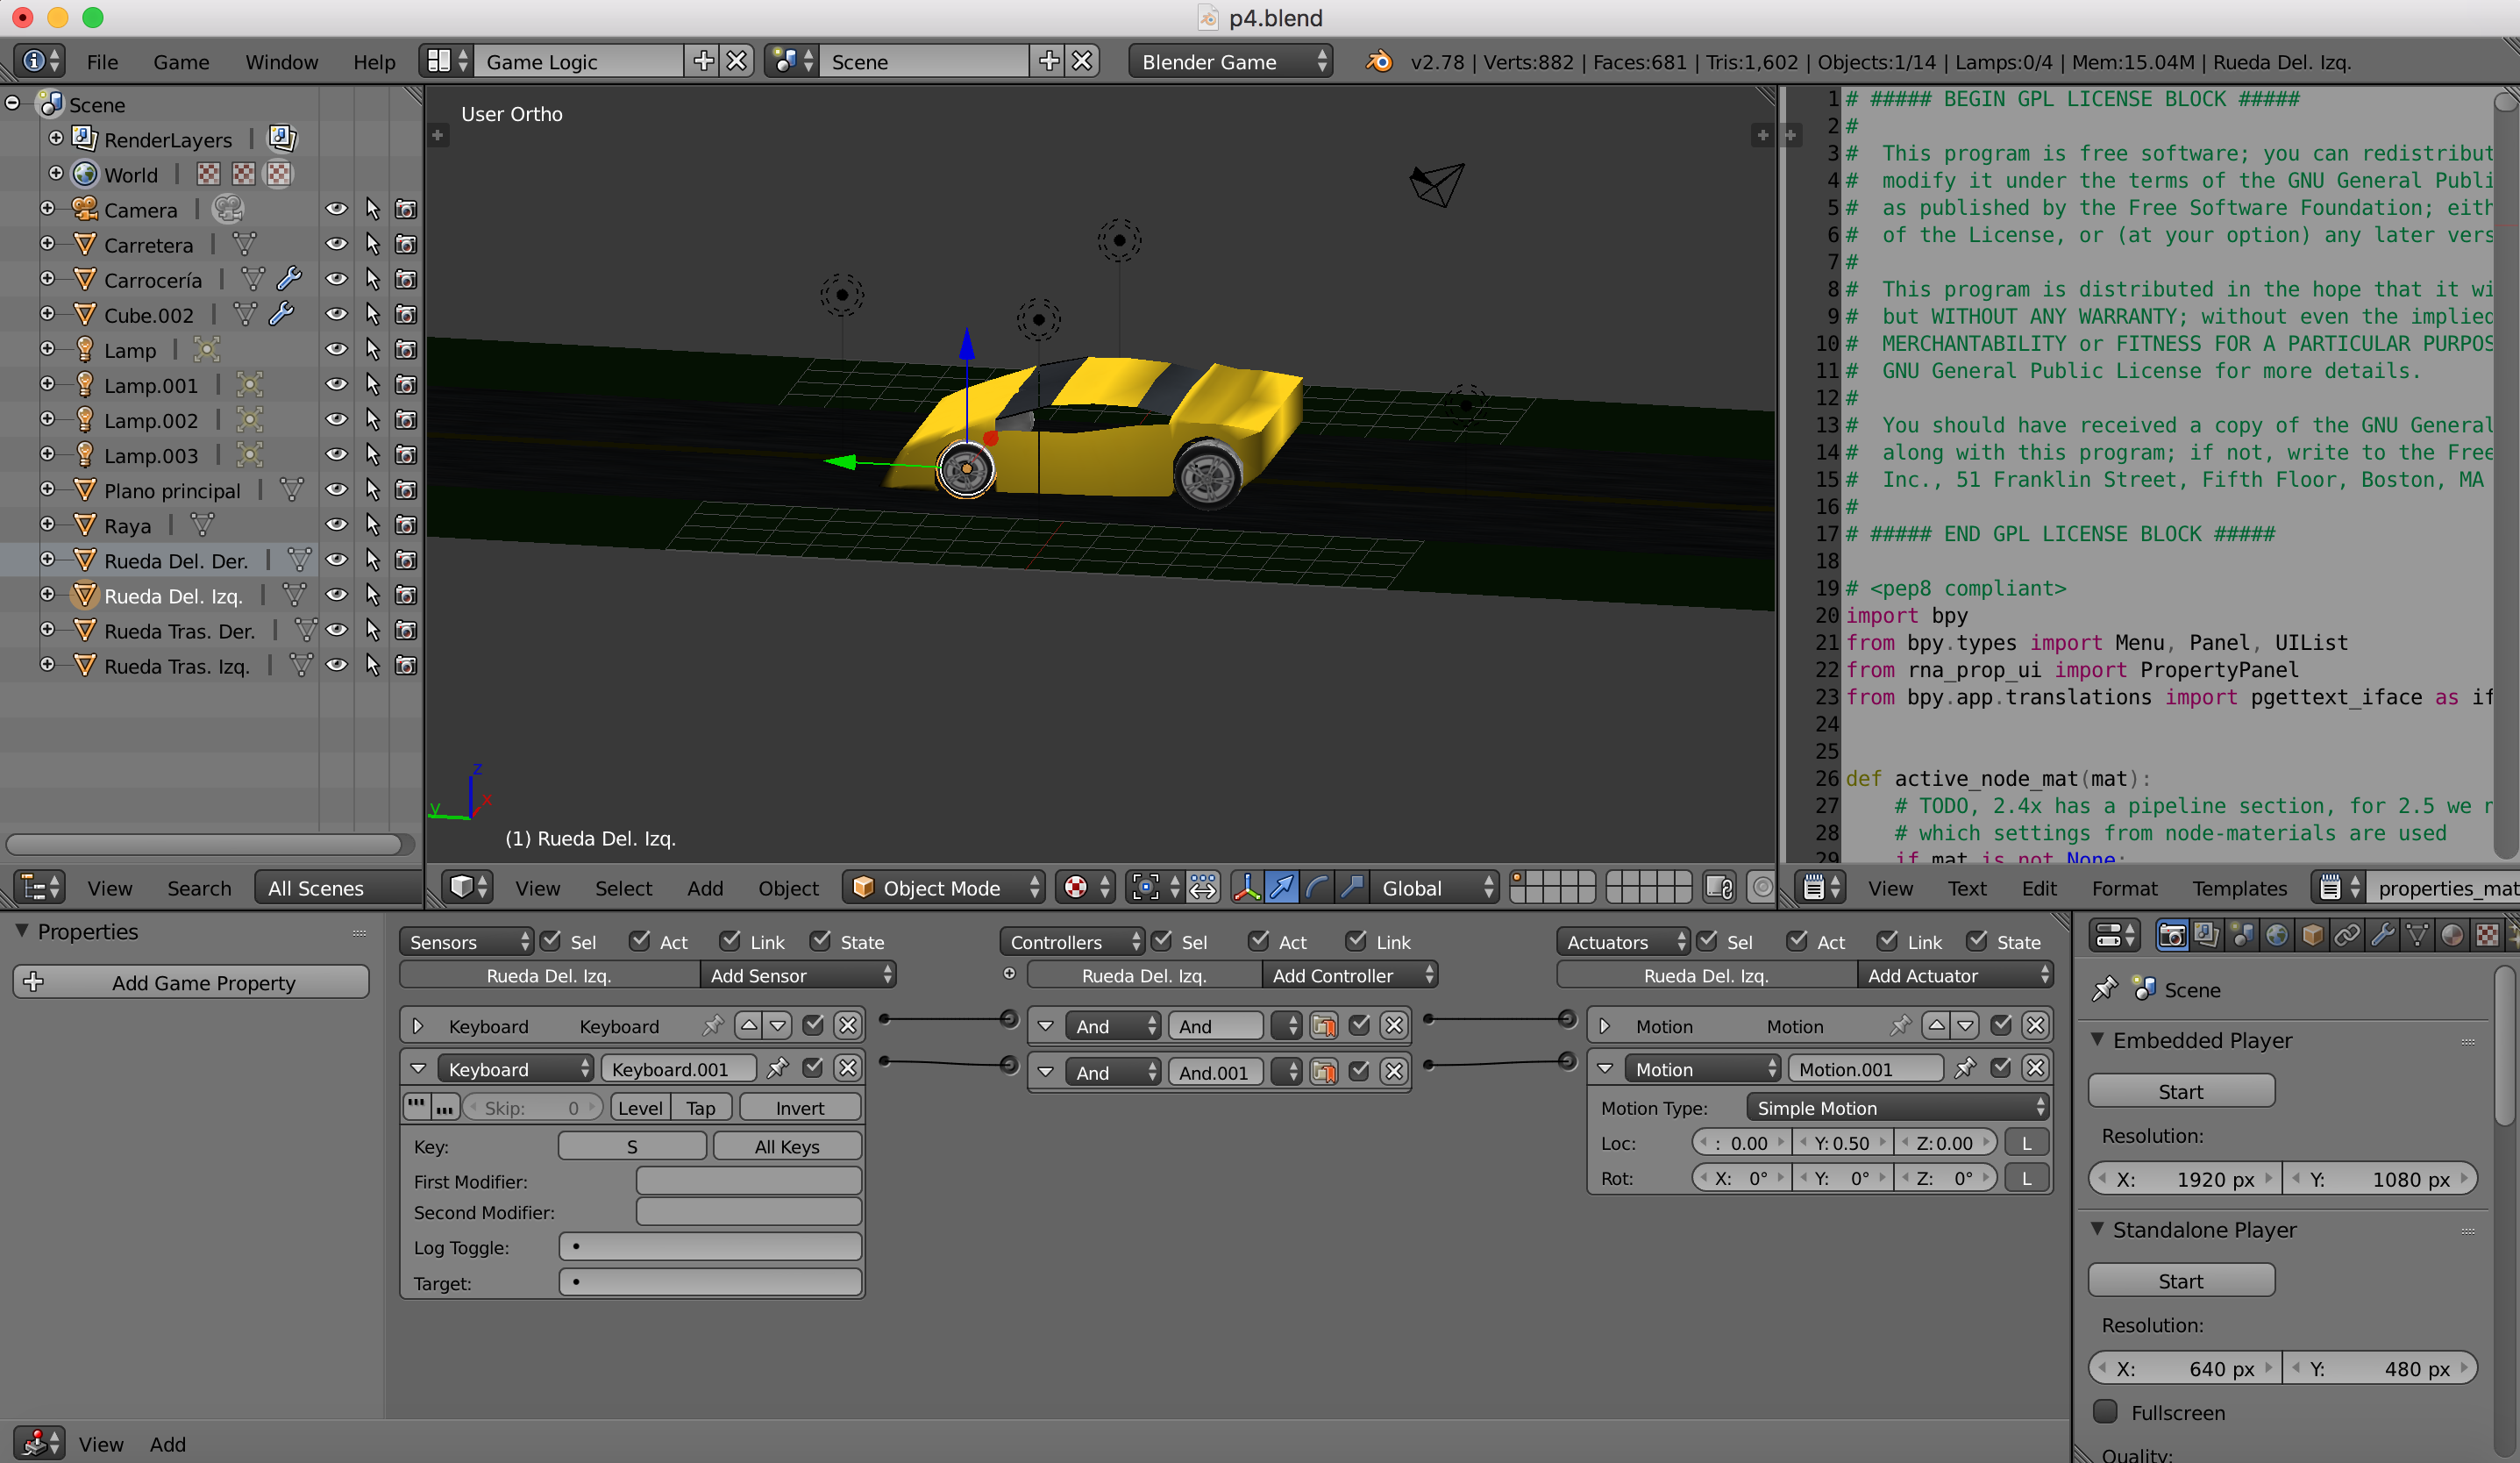
\includegraphics[width = 1.00\textwidth]{Imagenes/p4-img6}
 		\captionof{figure}{\label{fig:IPN}Añadiendo rotación en rueda delantera izquieda (II).} 
	\end{center} 
\end{figure}

\begin{figure}[H]
	\begin{center}
	 		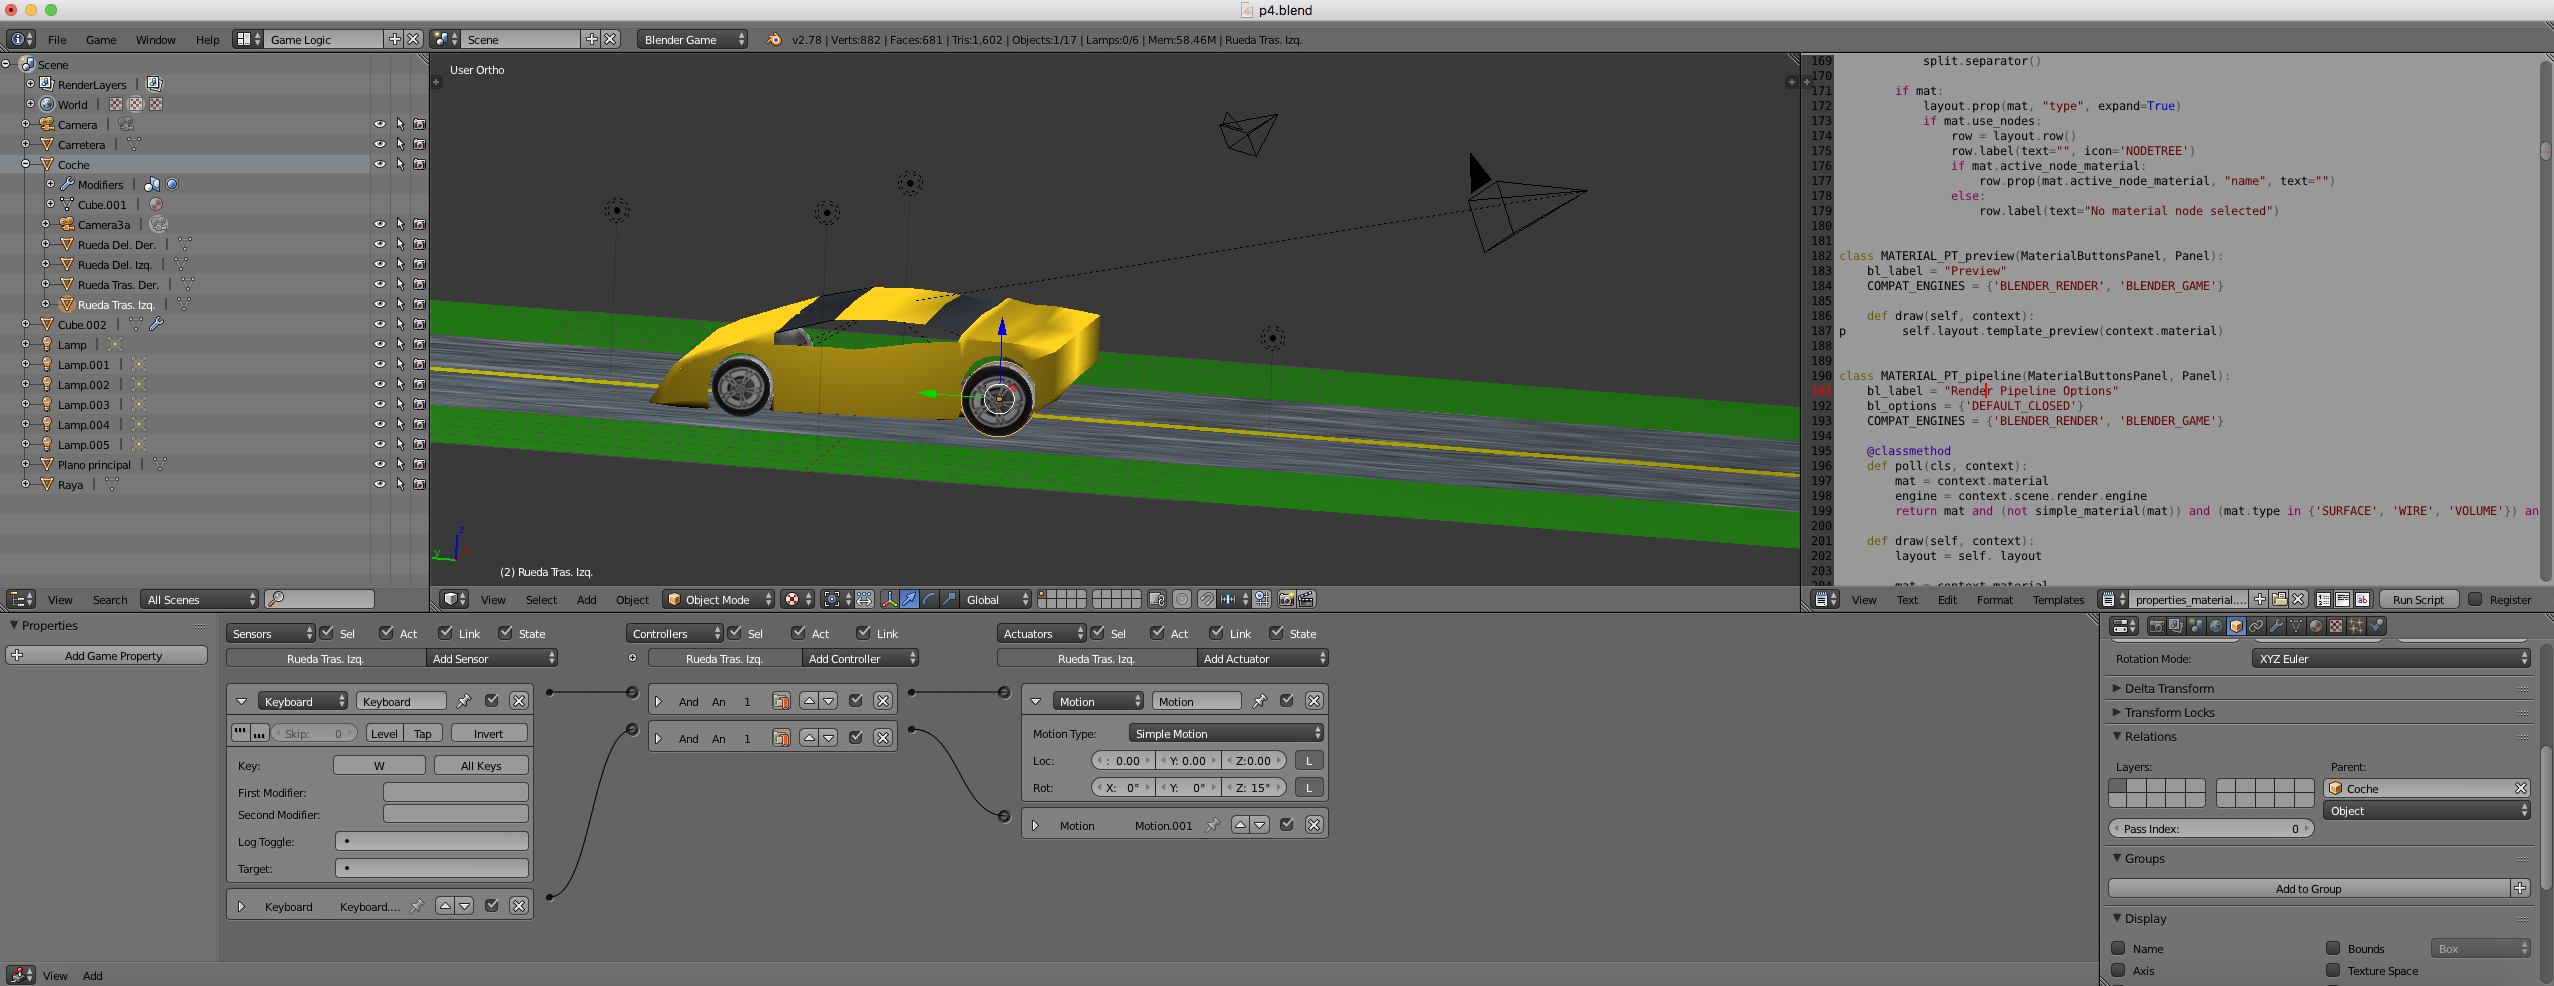
\includegraphics[width = 1.00\textwidth]{Imagenes/p4-img7}
 		\captionof{figure}{\label{fig:IPN}Añadiendo rotación en rueda trasera izquieda (I).} 
	\end{center} 
\end{figure}

\begin{figure}[H]
	\begin{center}
	 		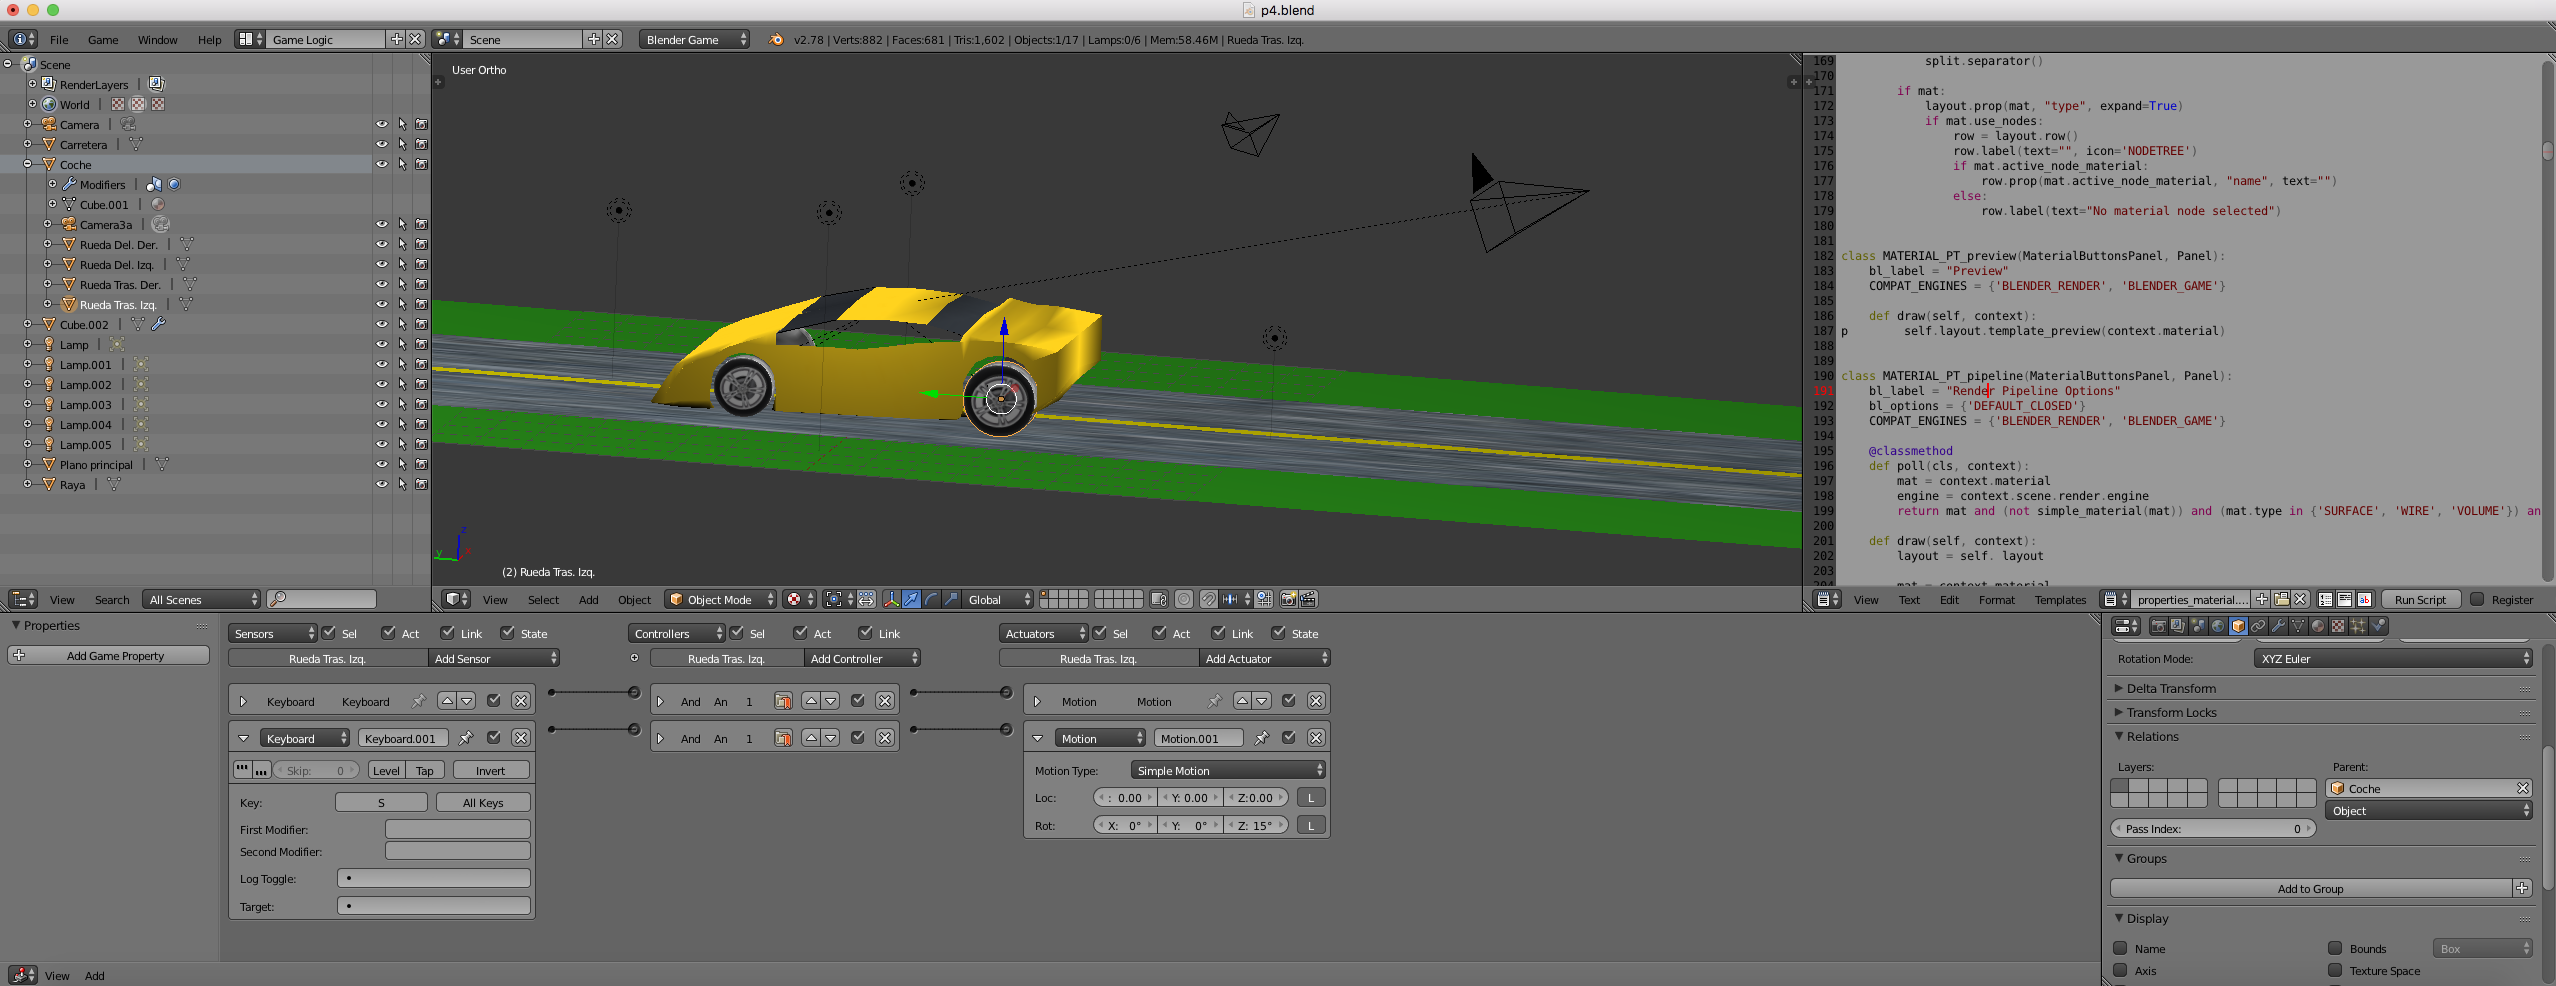
\includegraphics[width = 1.00\textwidth]{Imagenes/p4-img8}
 		\captionof{figure}{\label{fig:IPN}Añadiendo rotación en rueda trasera izquieda (II).} 
	\end{center} 
\end{figure}

\begin{figure}[H]
	\begin{center}
	 		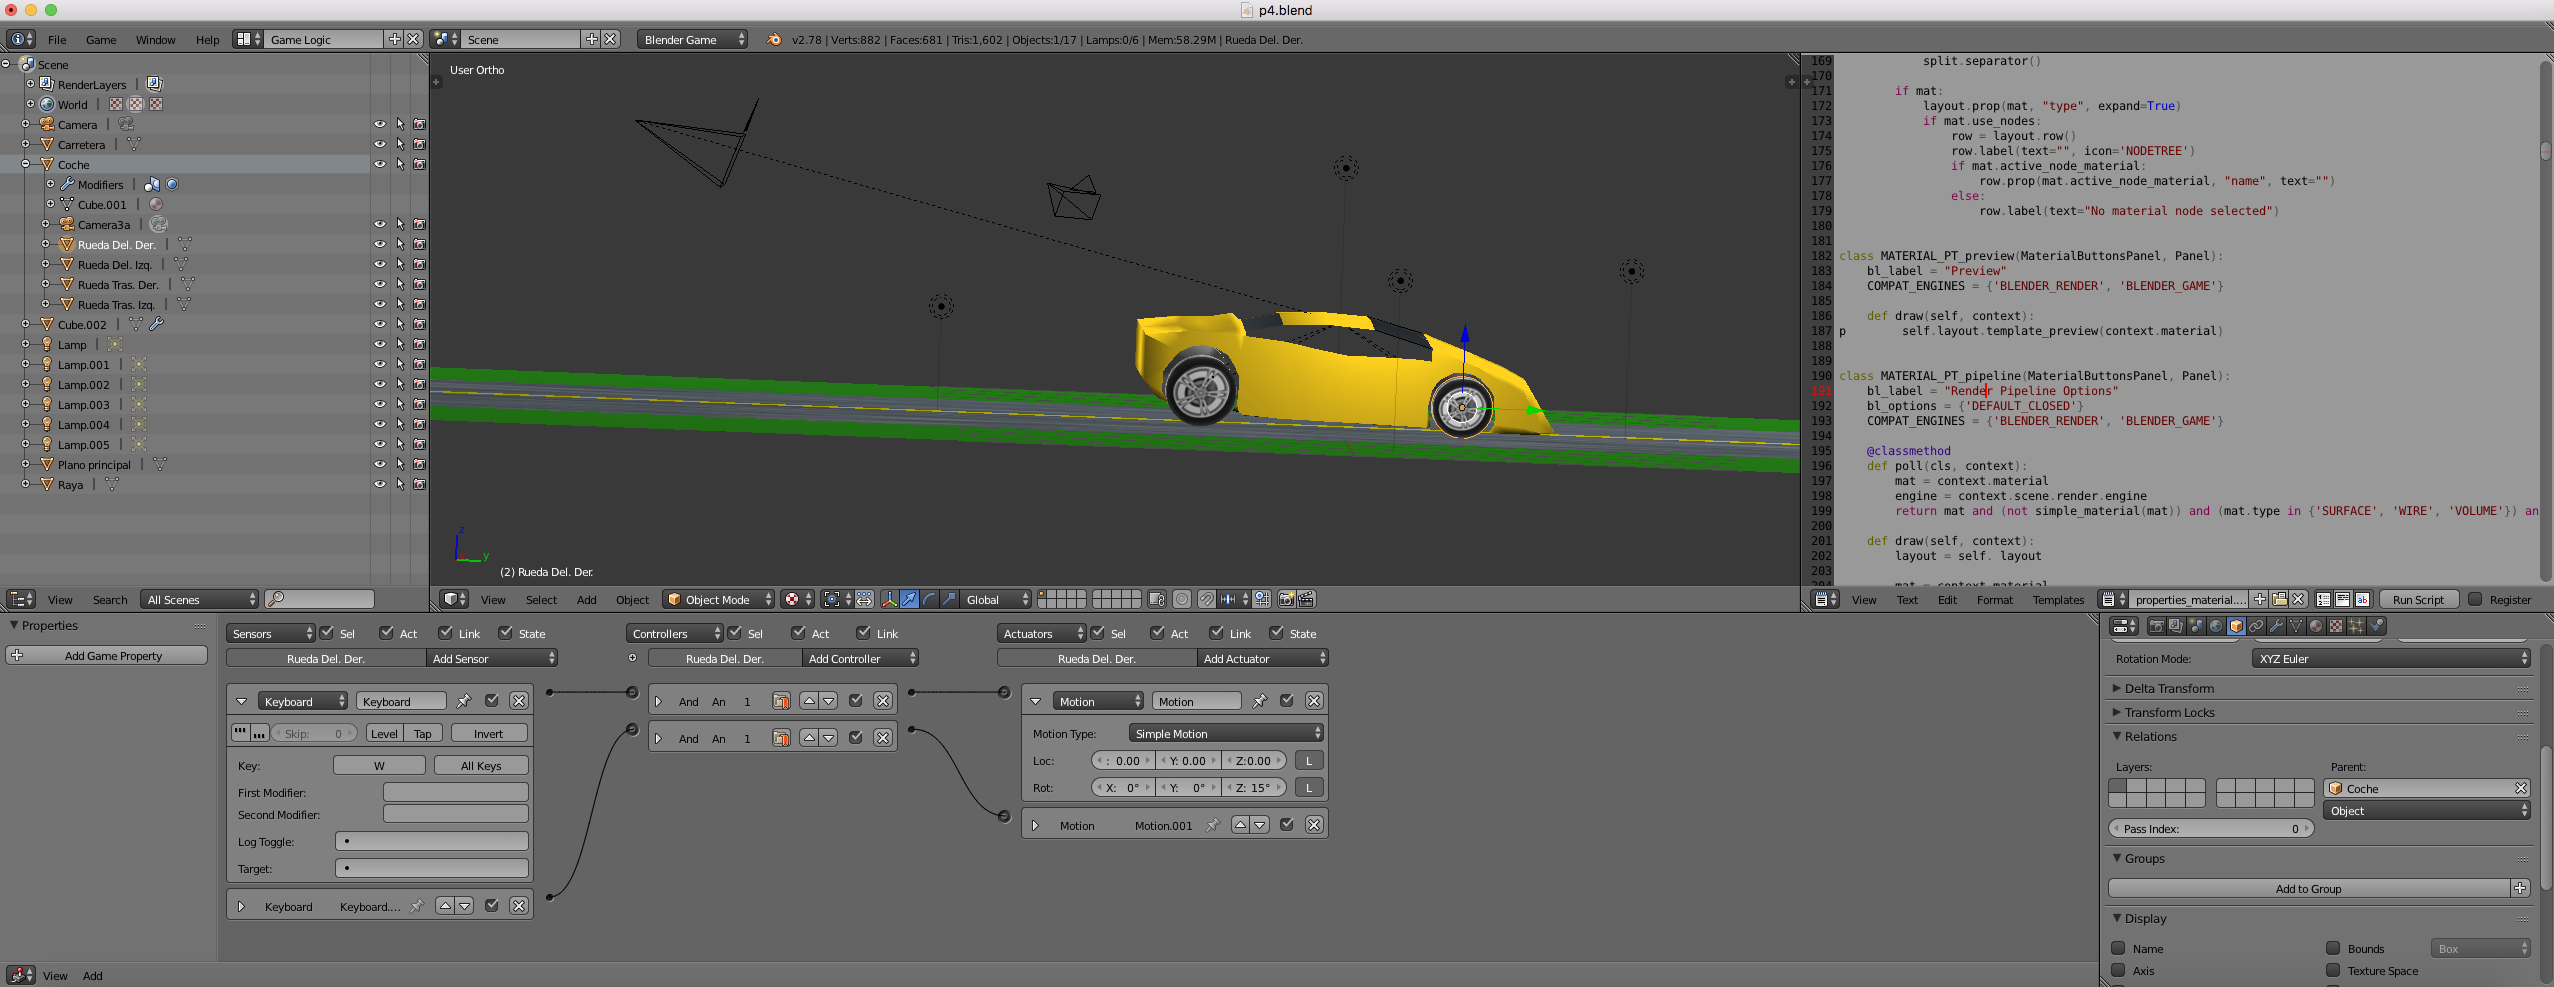
\includegraphics[width = 1.00\textwidth]{Imagenes/p4-img9}
 		\captionof{figure}{\label{fig:IPN}Añadiendo rotación en rueda delantera derecha (I).} 
	\end{center} 
\end{figure}

\begin{figure}[H]
	\begin{center}
	 		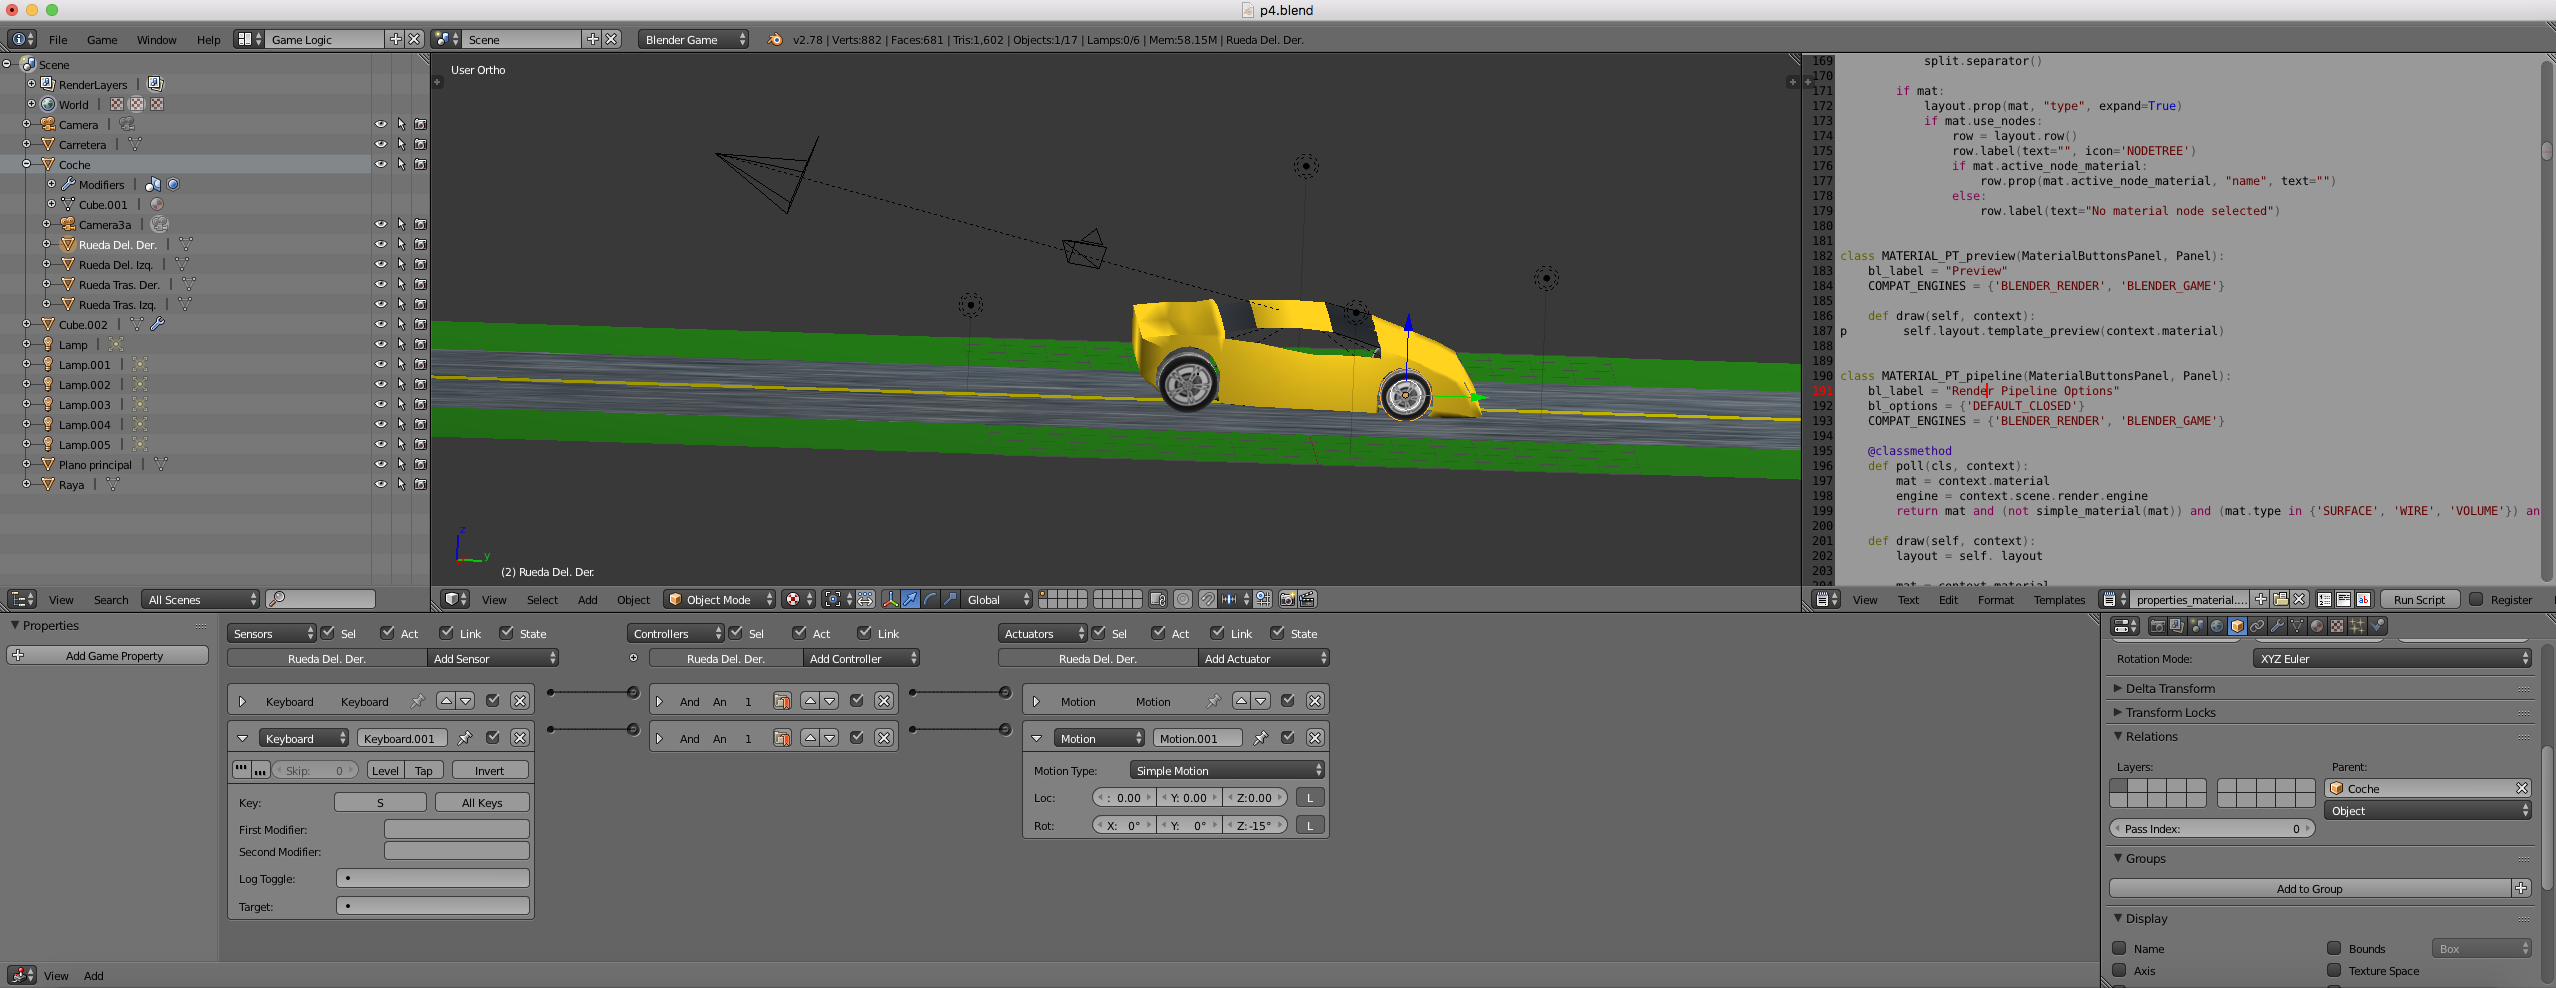
\includegraphics[width = 1.00\textwidth]{Imagenes/p4-img10}
 		\captionof{figure}{\label{fig:IPN}Añadiendo rotación en rueda delantera derecha (II).} 
	\end{center} 
\end{figure}

\begin{figure}[H]
	\begin{center}
	 		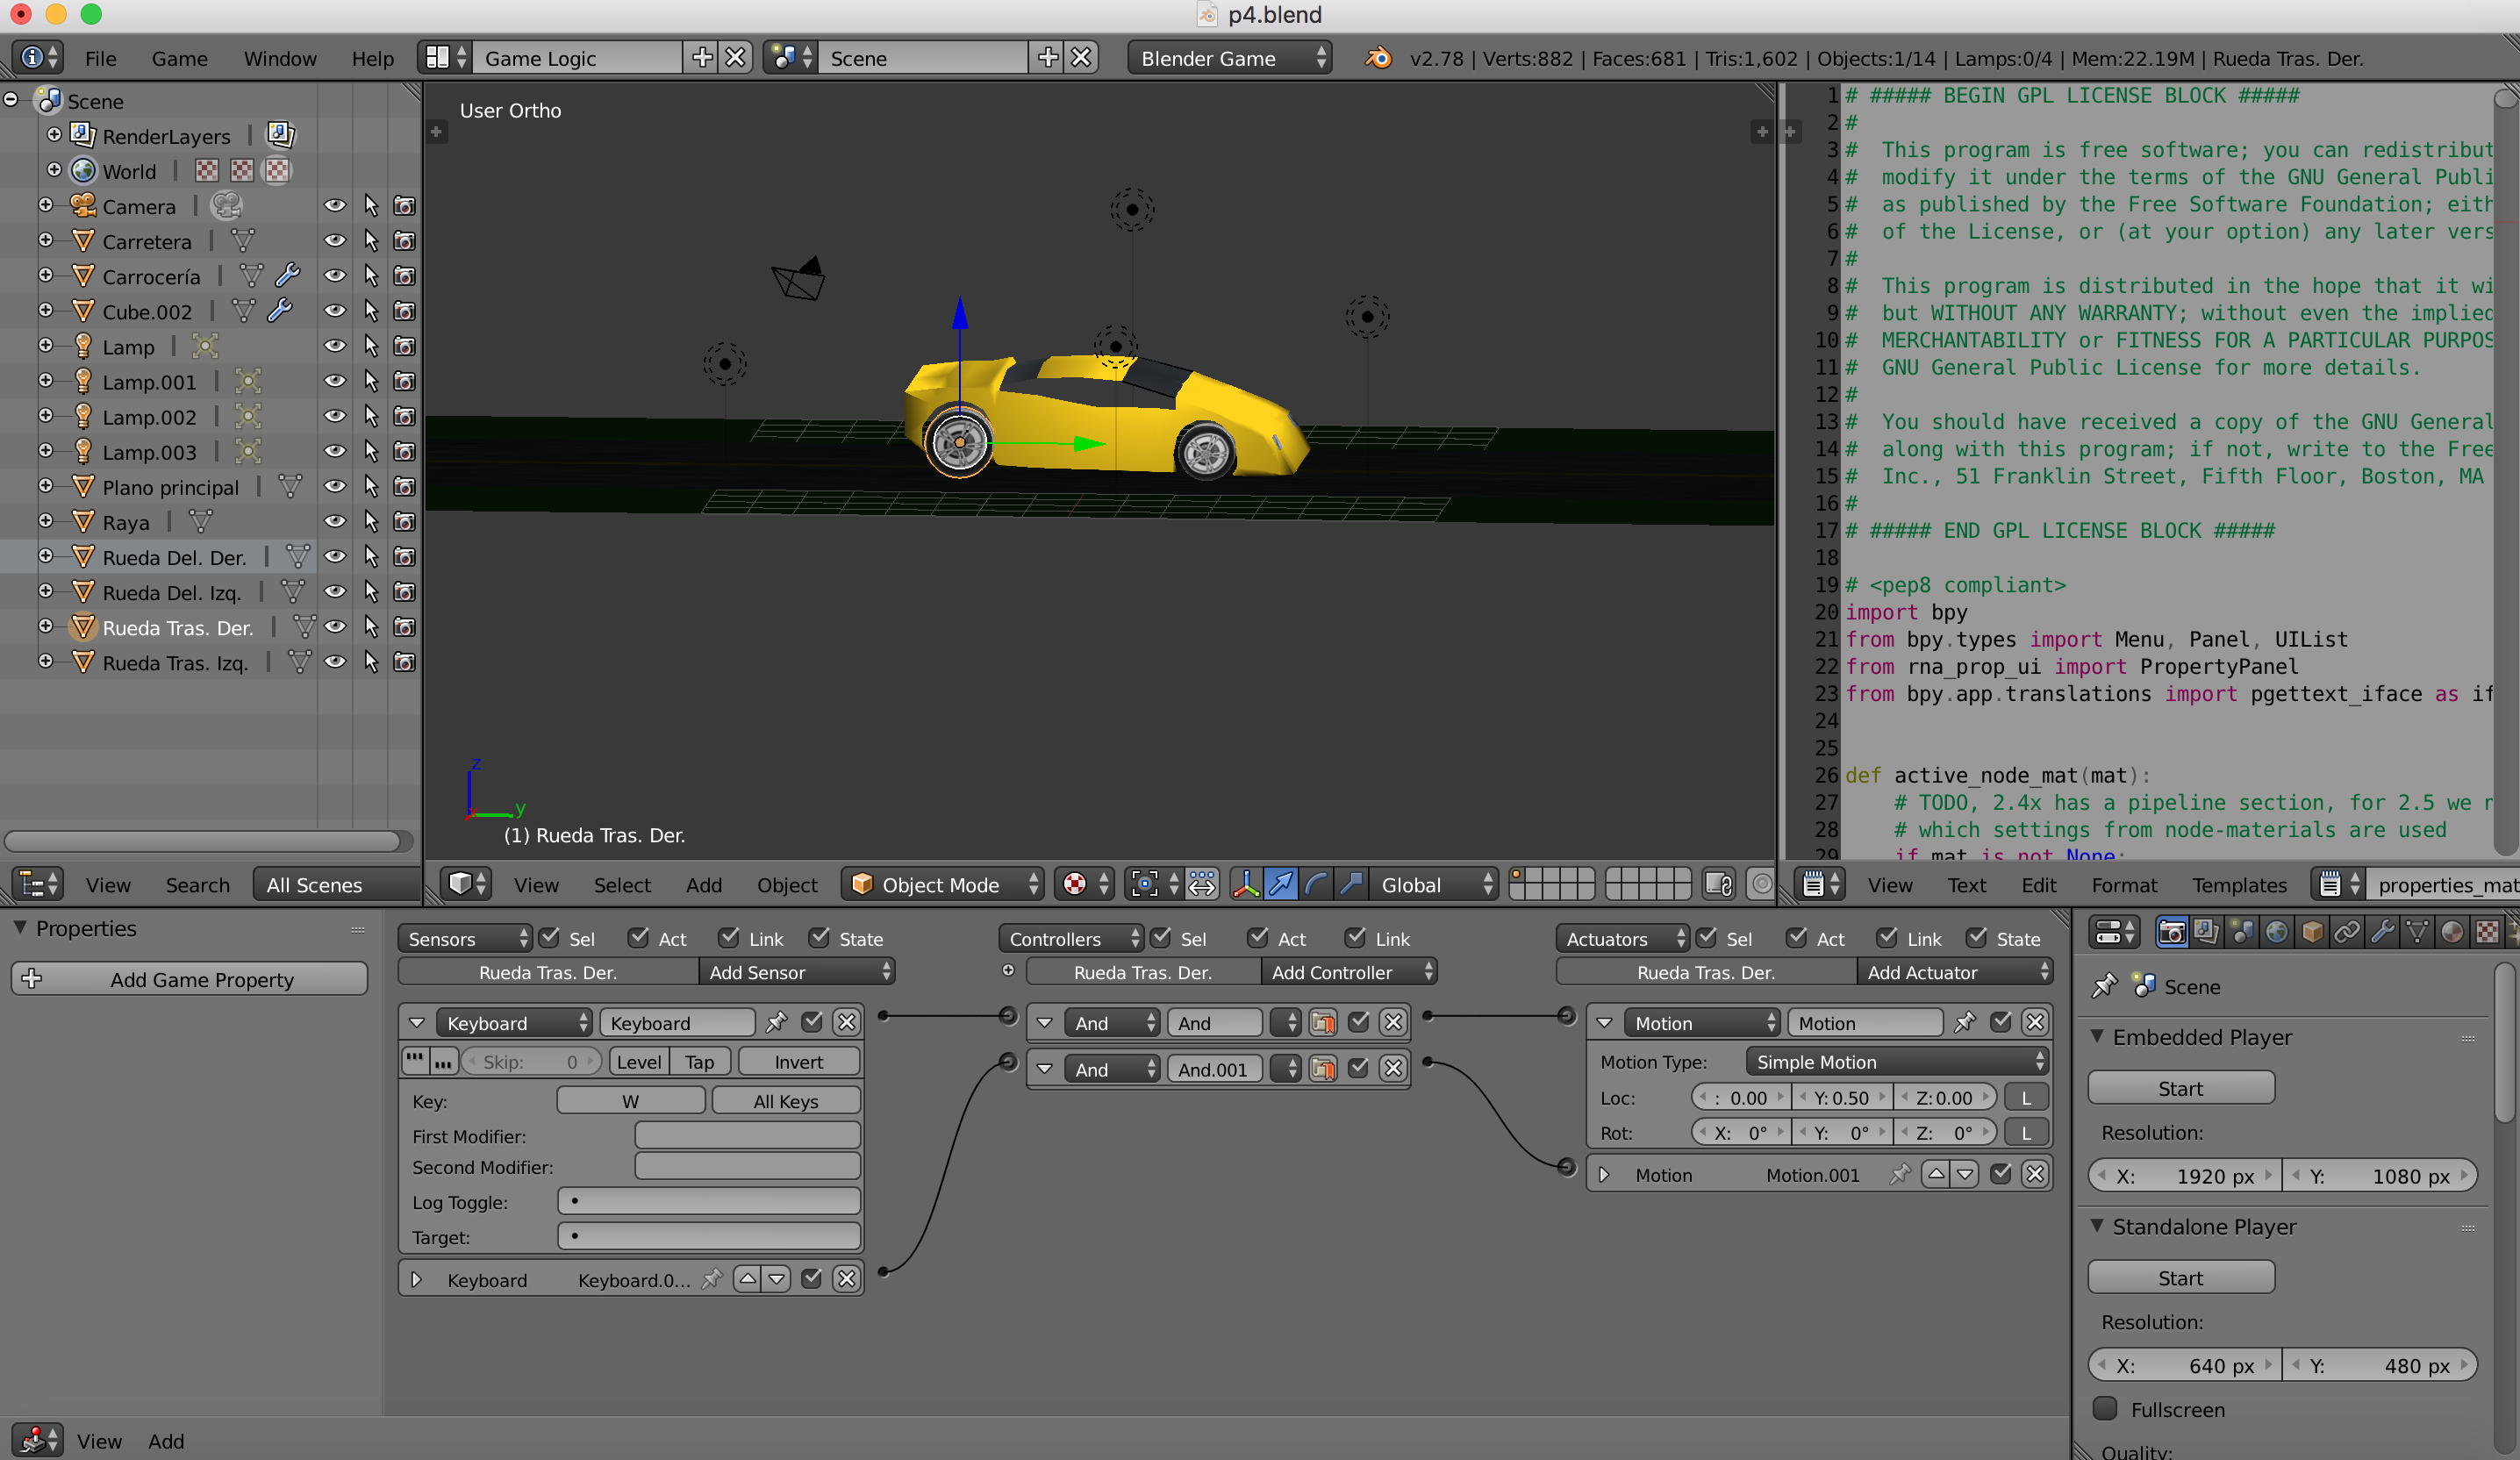
\includegraphics[width = 1.00\textwidth]{Imagenes/p4-img11}
 		\captionof{figure}{\label{fig:IPN}Añadiendo rotación en rueda trasera derecha (I).} 
	\end{center} 
\end{figure}

\begin{figure}[H]
	\begin{center}
	 		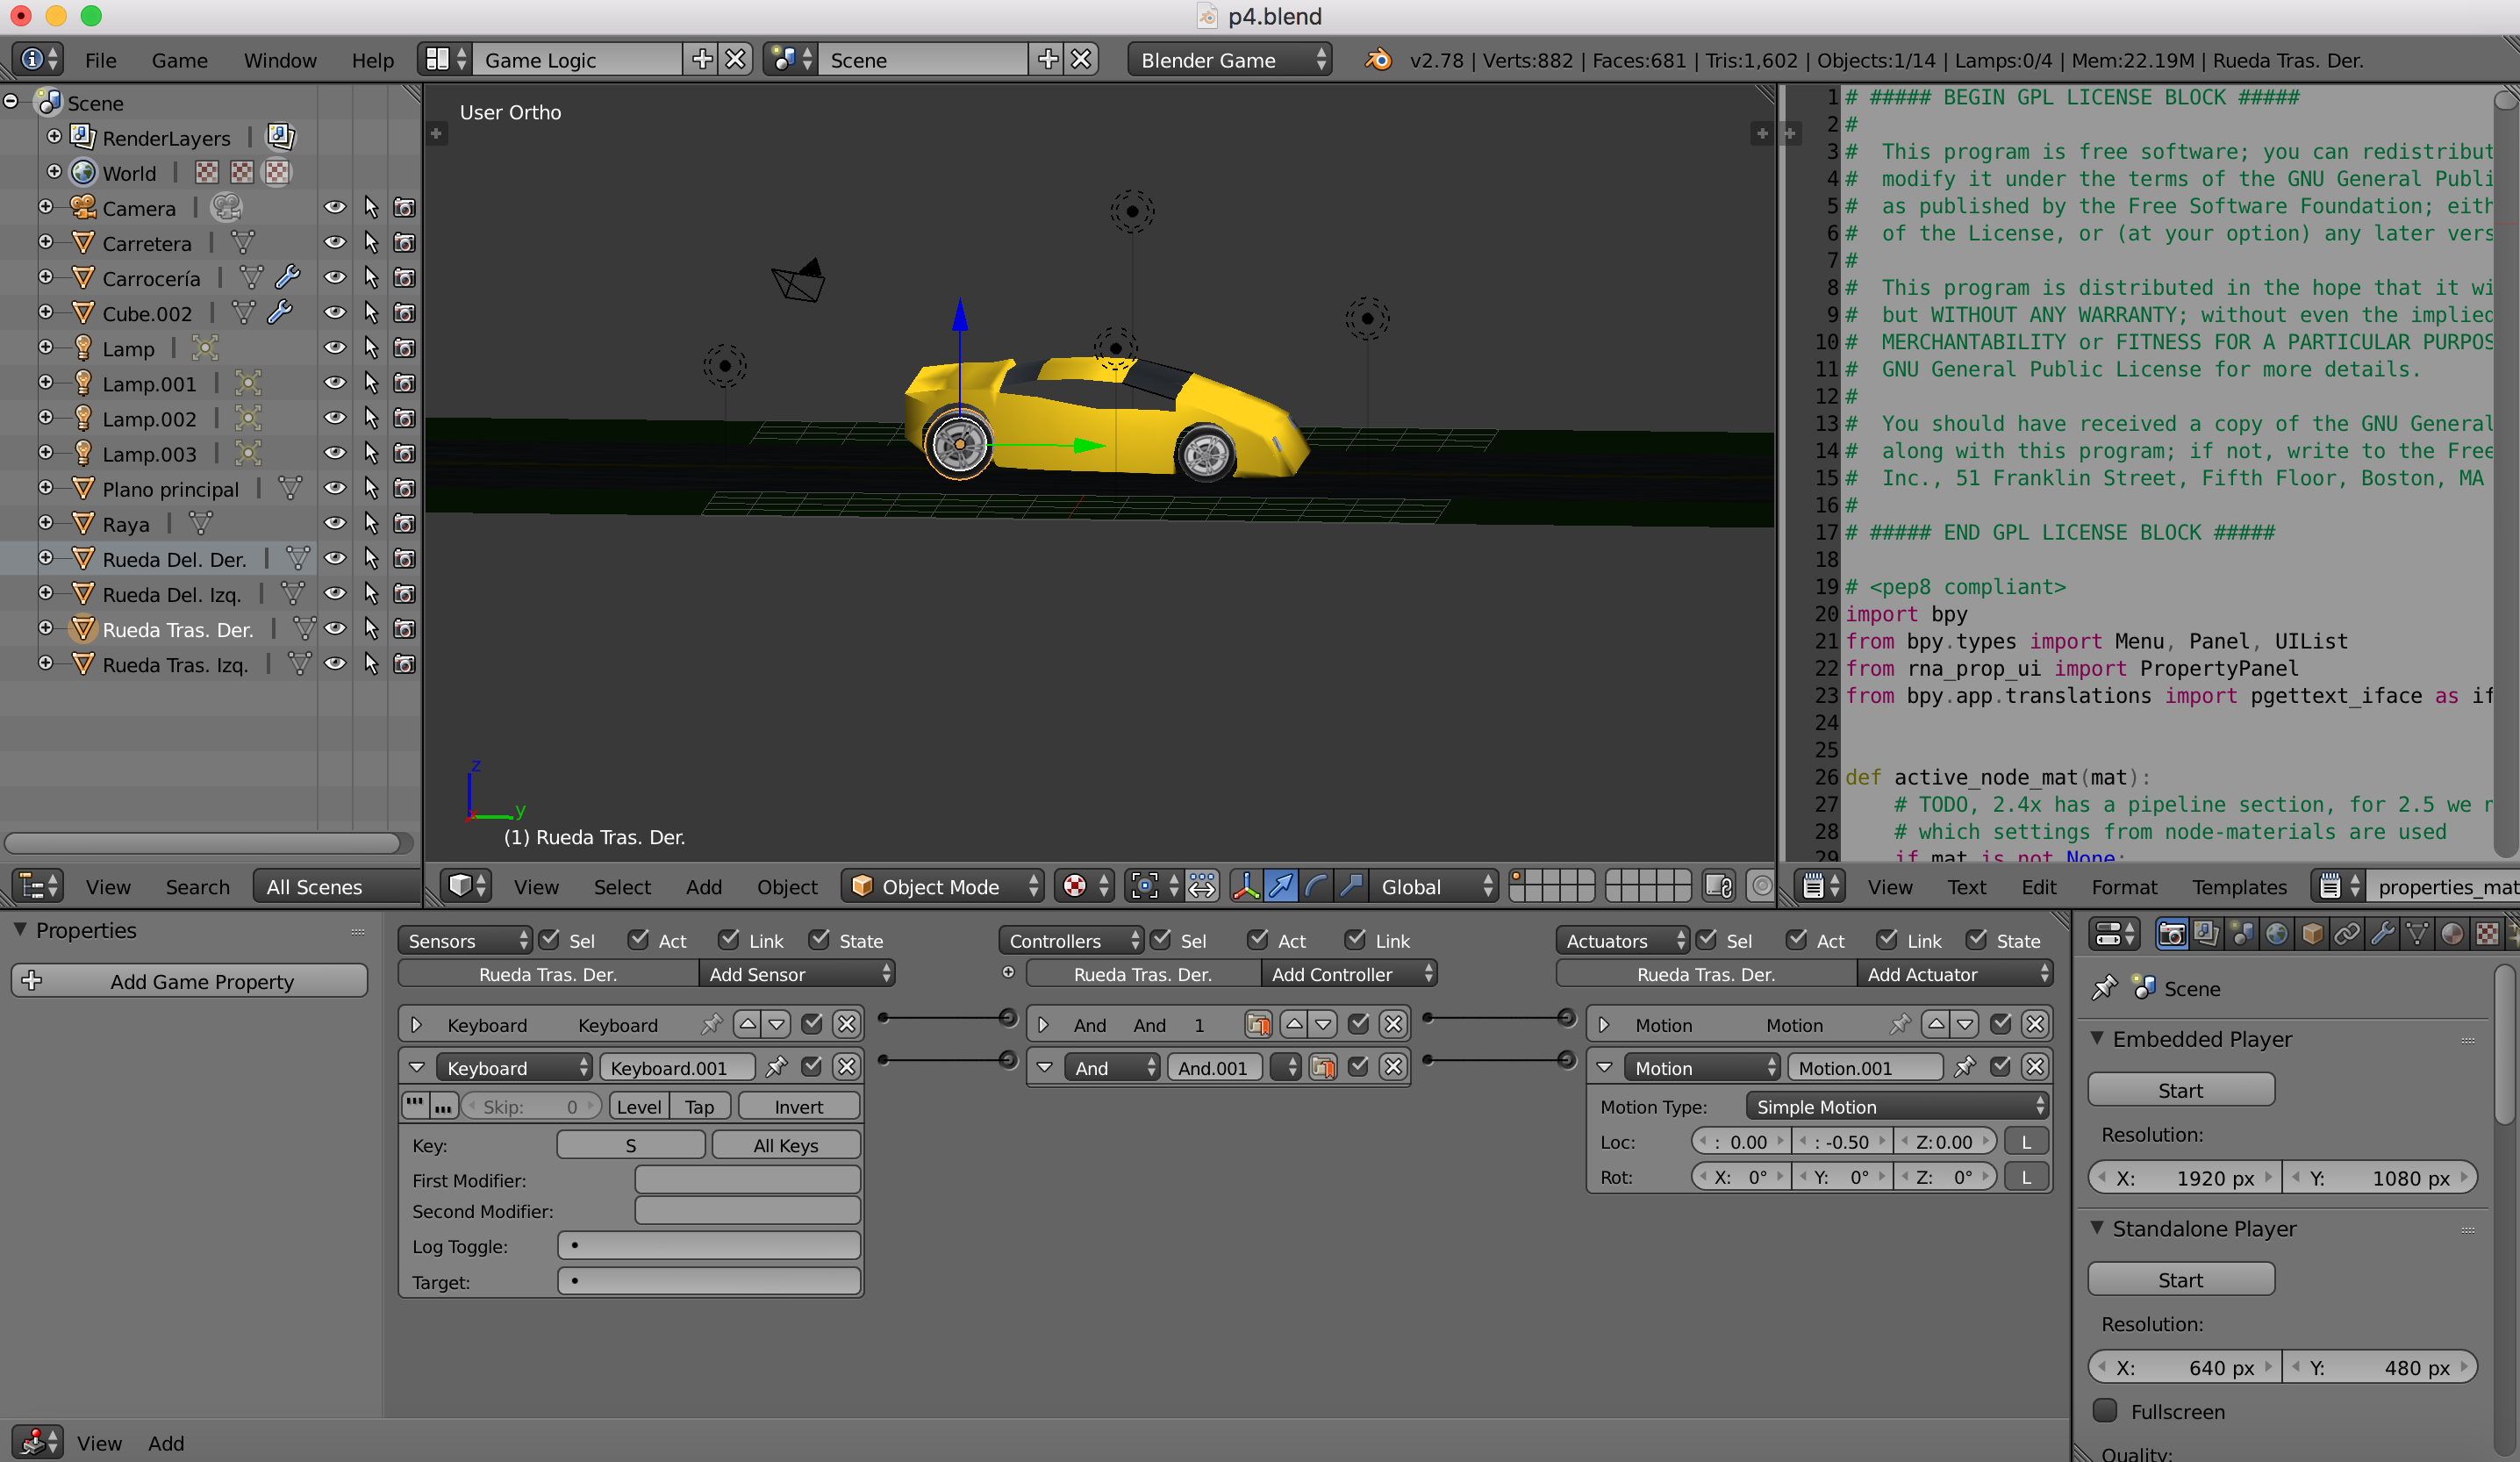
\includegraphics[width = 1.00\textwidth]{Imagenes/p4-img12}
 		\captionof{figure}{\label{fig:IPN}Añadiendo rotación en rueda trasera derecha (II).} 
	\end{center} 
\end{figure}



\subsection{Movimiento de cámara.}
Para hacer que la cámara siga al coche lo primero que vamos a hacer es añadir una nueva cámara ``Camera3a'' y ajustarla para posicionarla detrás del mismo como se ve en la siguiente imagen. \\

\begin{figure}[H]
	\begin{center}
	 		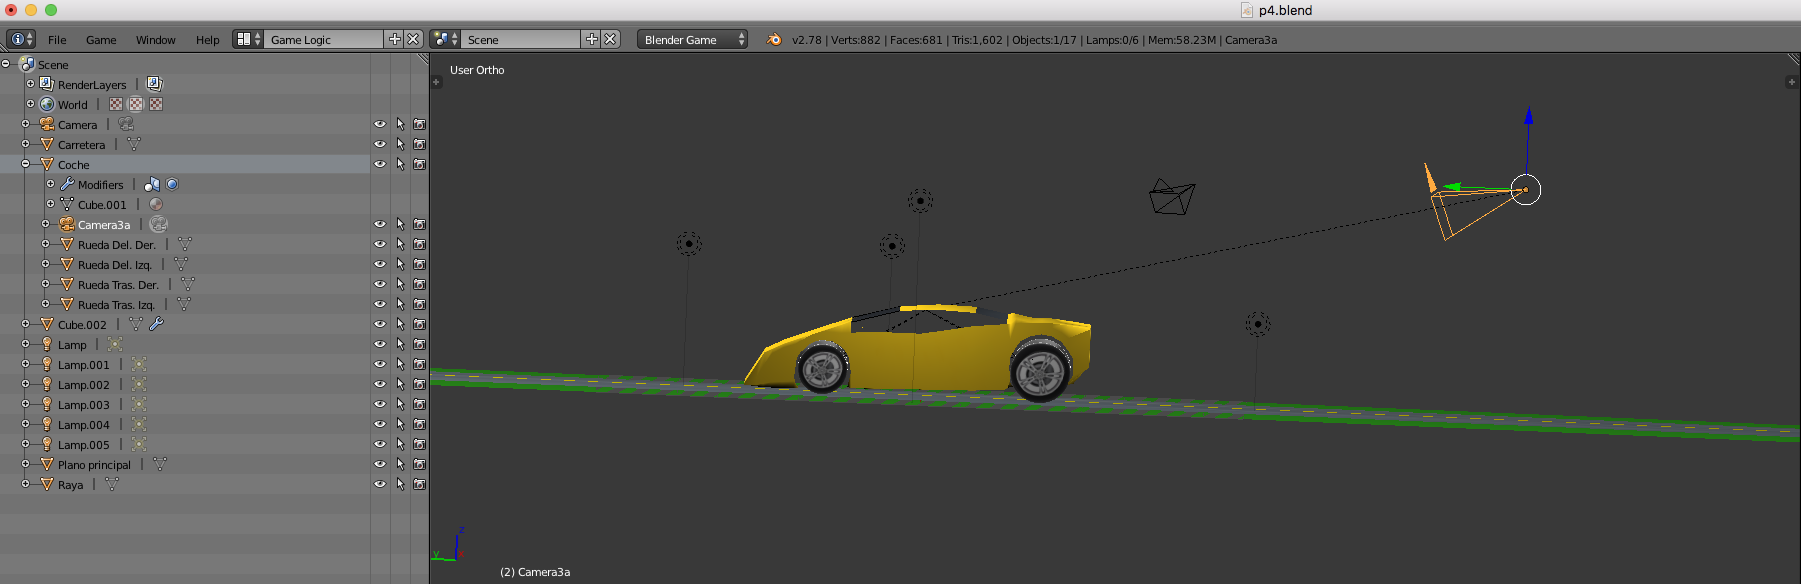
\includegraphics[width = 1.00\textwidth]{Imagenes/p4-img13}
 		\captionof{figure}{\label{fig:IPN}Añadiendo cámara y posicionándola.} 
	\end{center} 
\end{figure}

Lo siguiente que tenemos que hacer es emparentar la nueva cámara añadida al objeto ``Coche'' de modo 	que éste sea su padre.\\

\begin{figure}[H]
	\begin{center}
	 		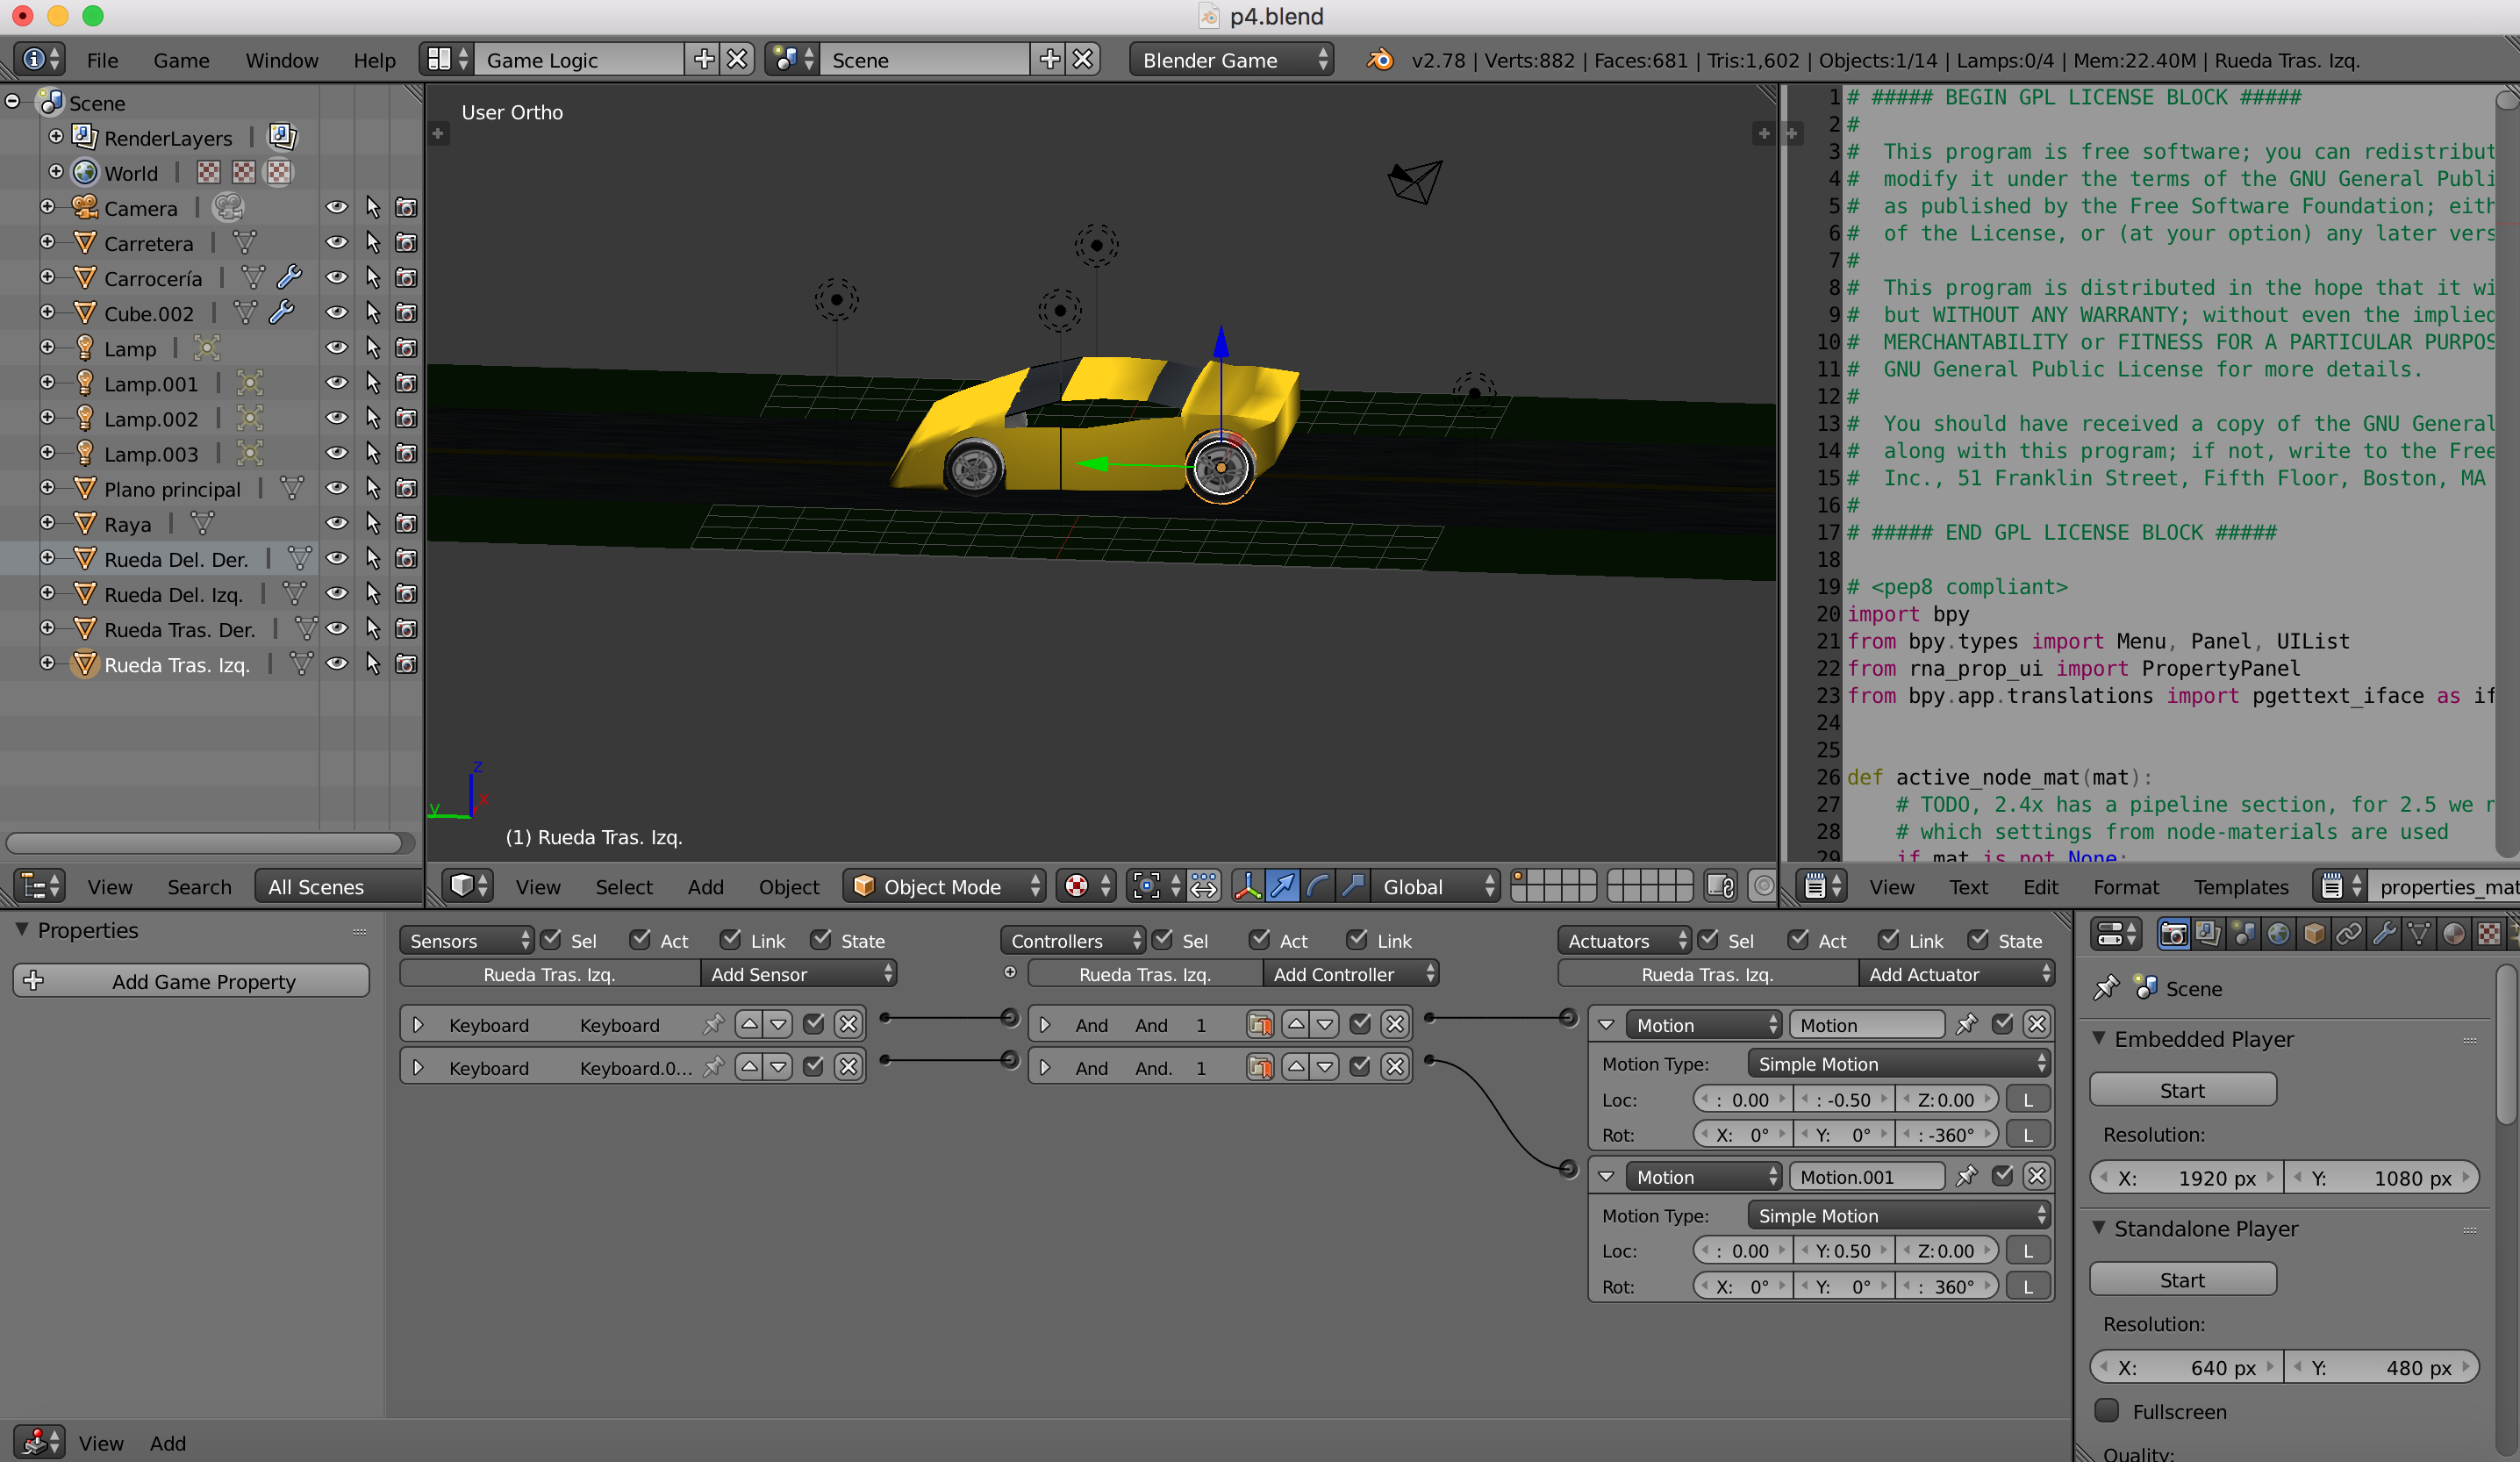
\includegraphics[width = 1.00\textwidth]{Imagenes/p4-img14}
 		\captionof{figure}{\label{fig:IPN}Emparentando objetos Camera3a y Coche.} 
	\end{center} 
\end{figure}

Con la cámara ``Camera3a'' y el objeto ``Coche'' emparentados, lo siguiente es añadirle un sensor, controlador y actuador a dicha cámara para que siga al objeto ``Coche'' cuando este se encuentre en movimiento. Para ello añadimos un sensor de tipo ``Delay'' el cual dejaremos los parámetros por defecto y un actuador de tipo ``Mouse'' en modo ``Look'', a este componente le dejamos el valor mínimo y máximo de giro sobre el eje Y de -90º y 90º respectivamente, y le añadimos un ángulo mínimo de -30º y máximo de 30º para el eje X. \\

\begin{figure}[H]
	\begin{center}
	 		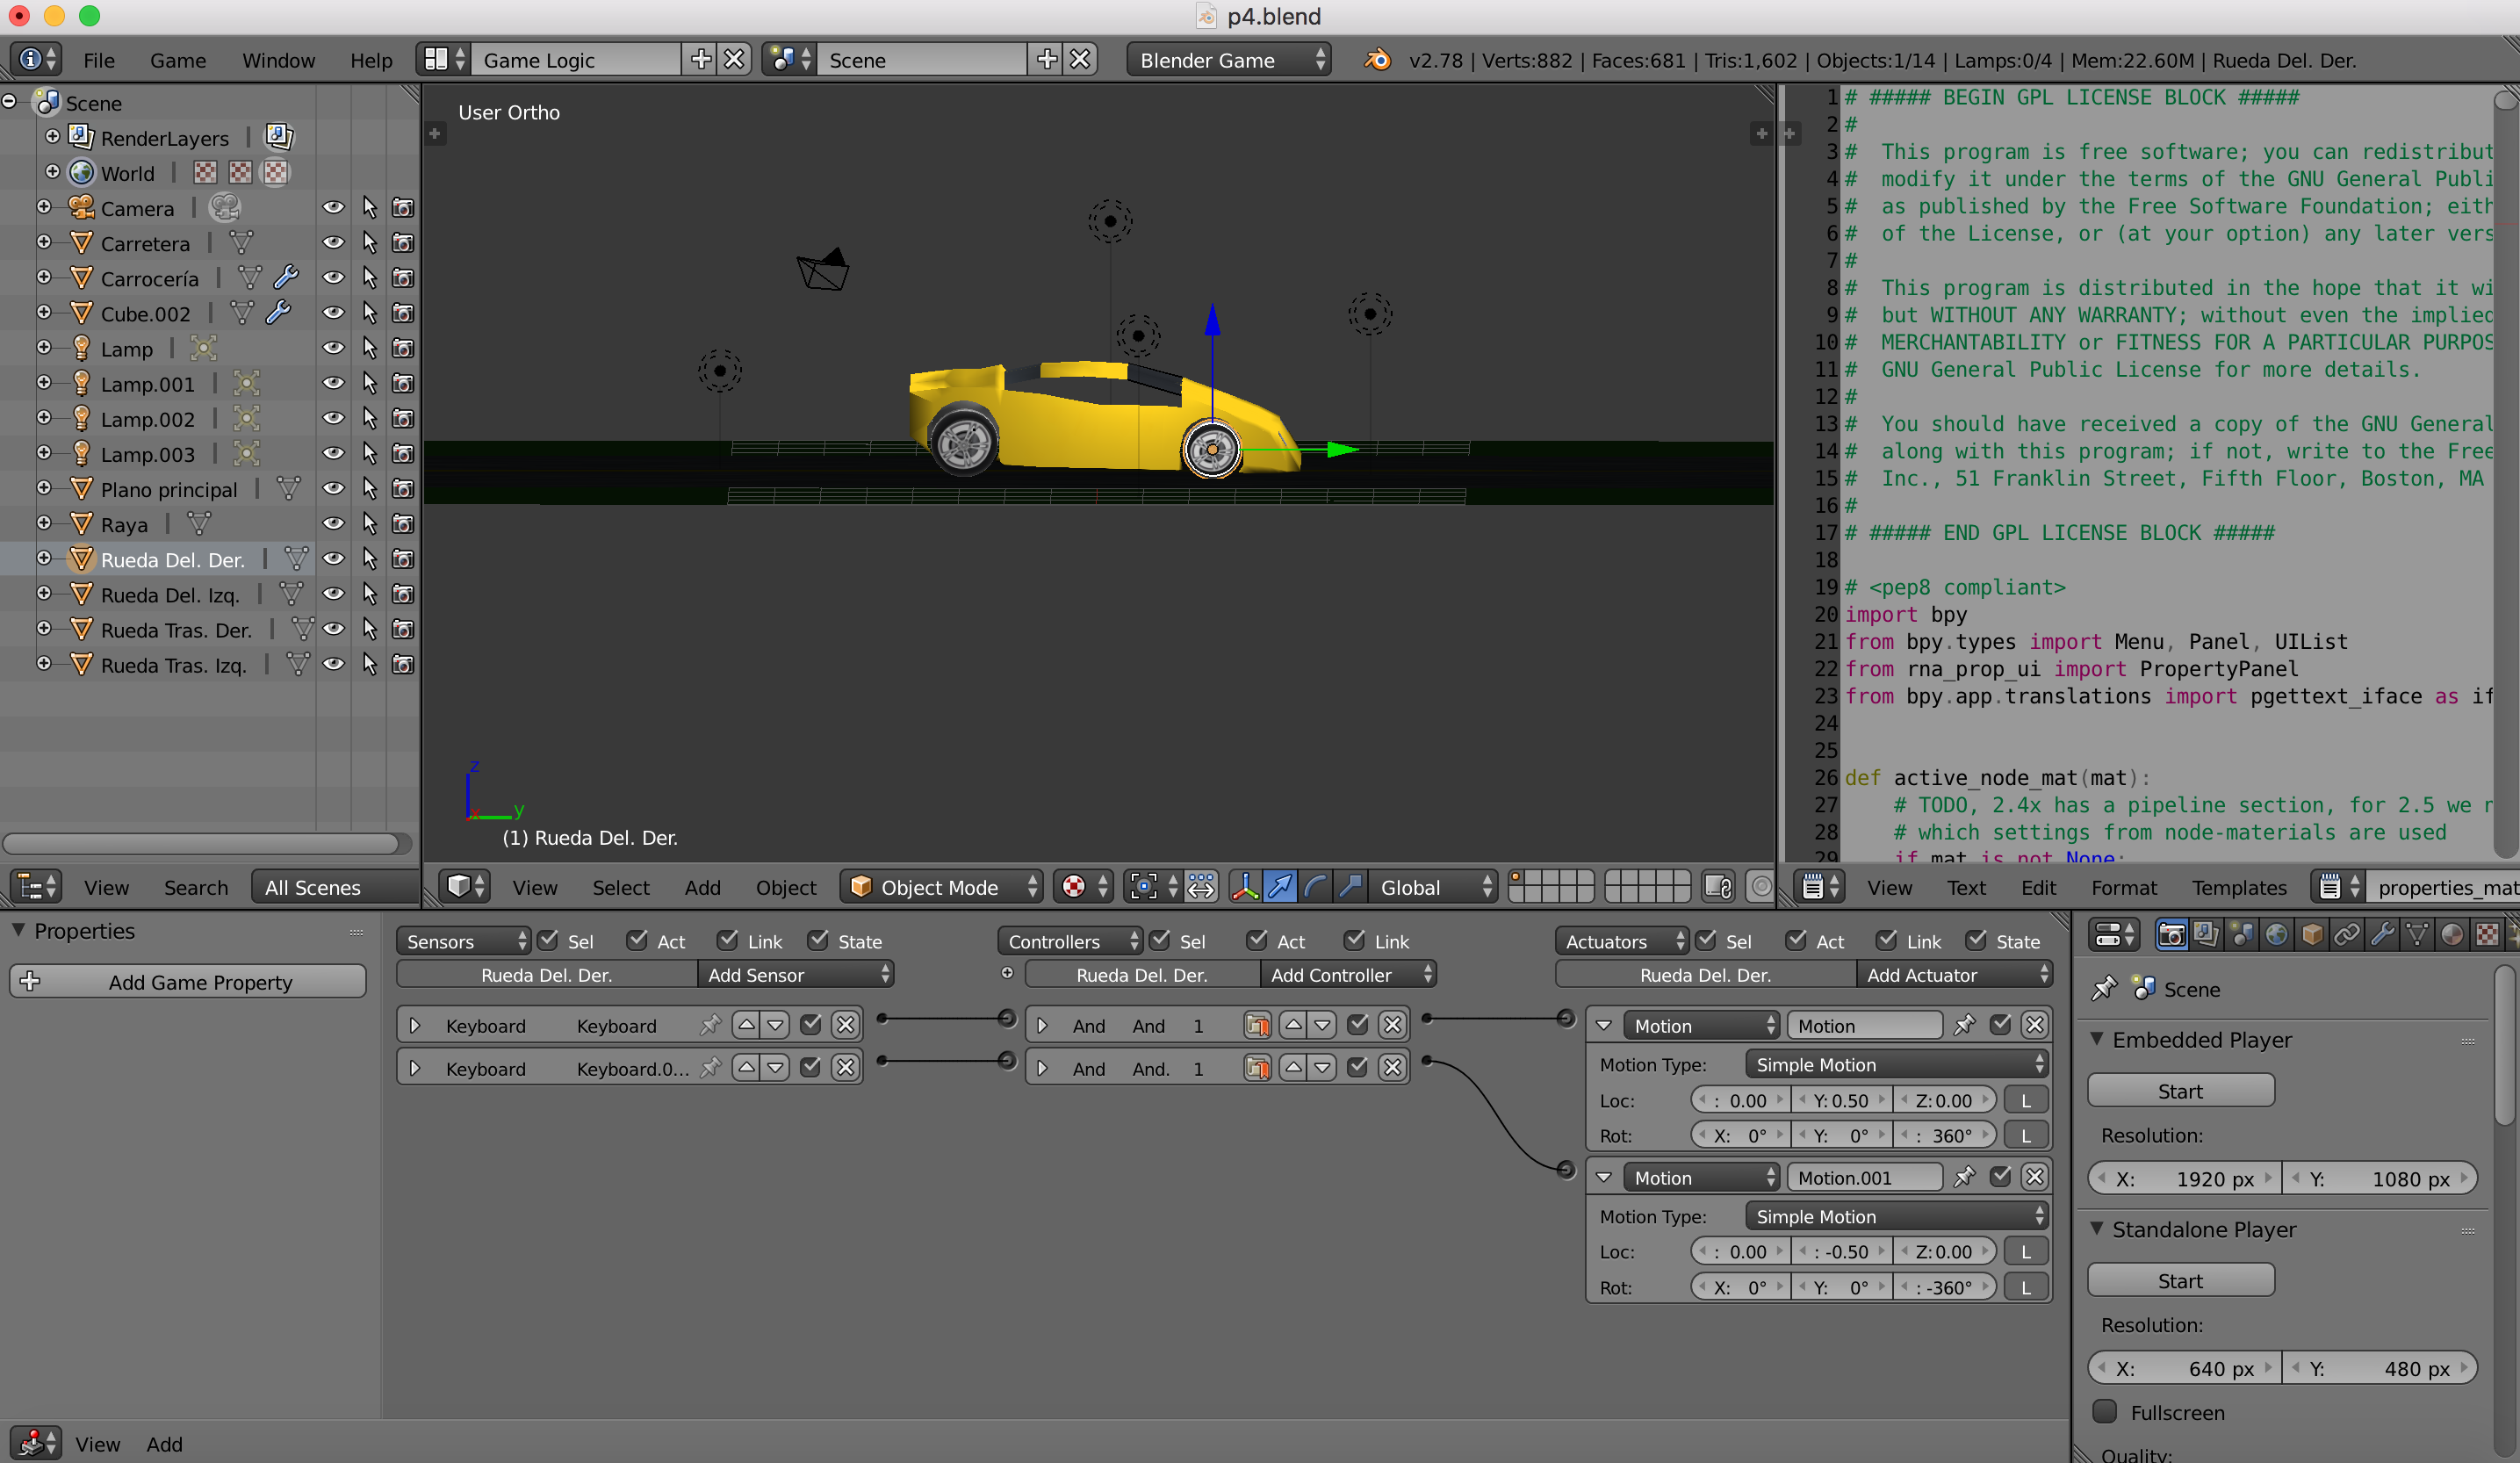
\includegraphics[width = 1.00\textwidth]{Imagenes/p4-img15}
 		\captionof{figure}{\label{fig:IPN}Añadiendo sensor, controlador y actuador al objeto ``Camera3a''  .} 
	\end{center} 
\end{figure}

Con todo ya configurado sólo queda pulsar la tecla 0 para poner la vista en ``Perspectiva'' para obtener la vista de la cámara activa (la que hemos añadido) y pulaE la tecla P para comenzar con la ejecución de la interacción.\\

\begin{figure}[H]
	\begin{center}
	 		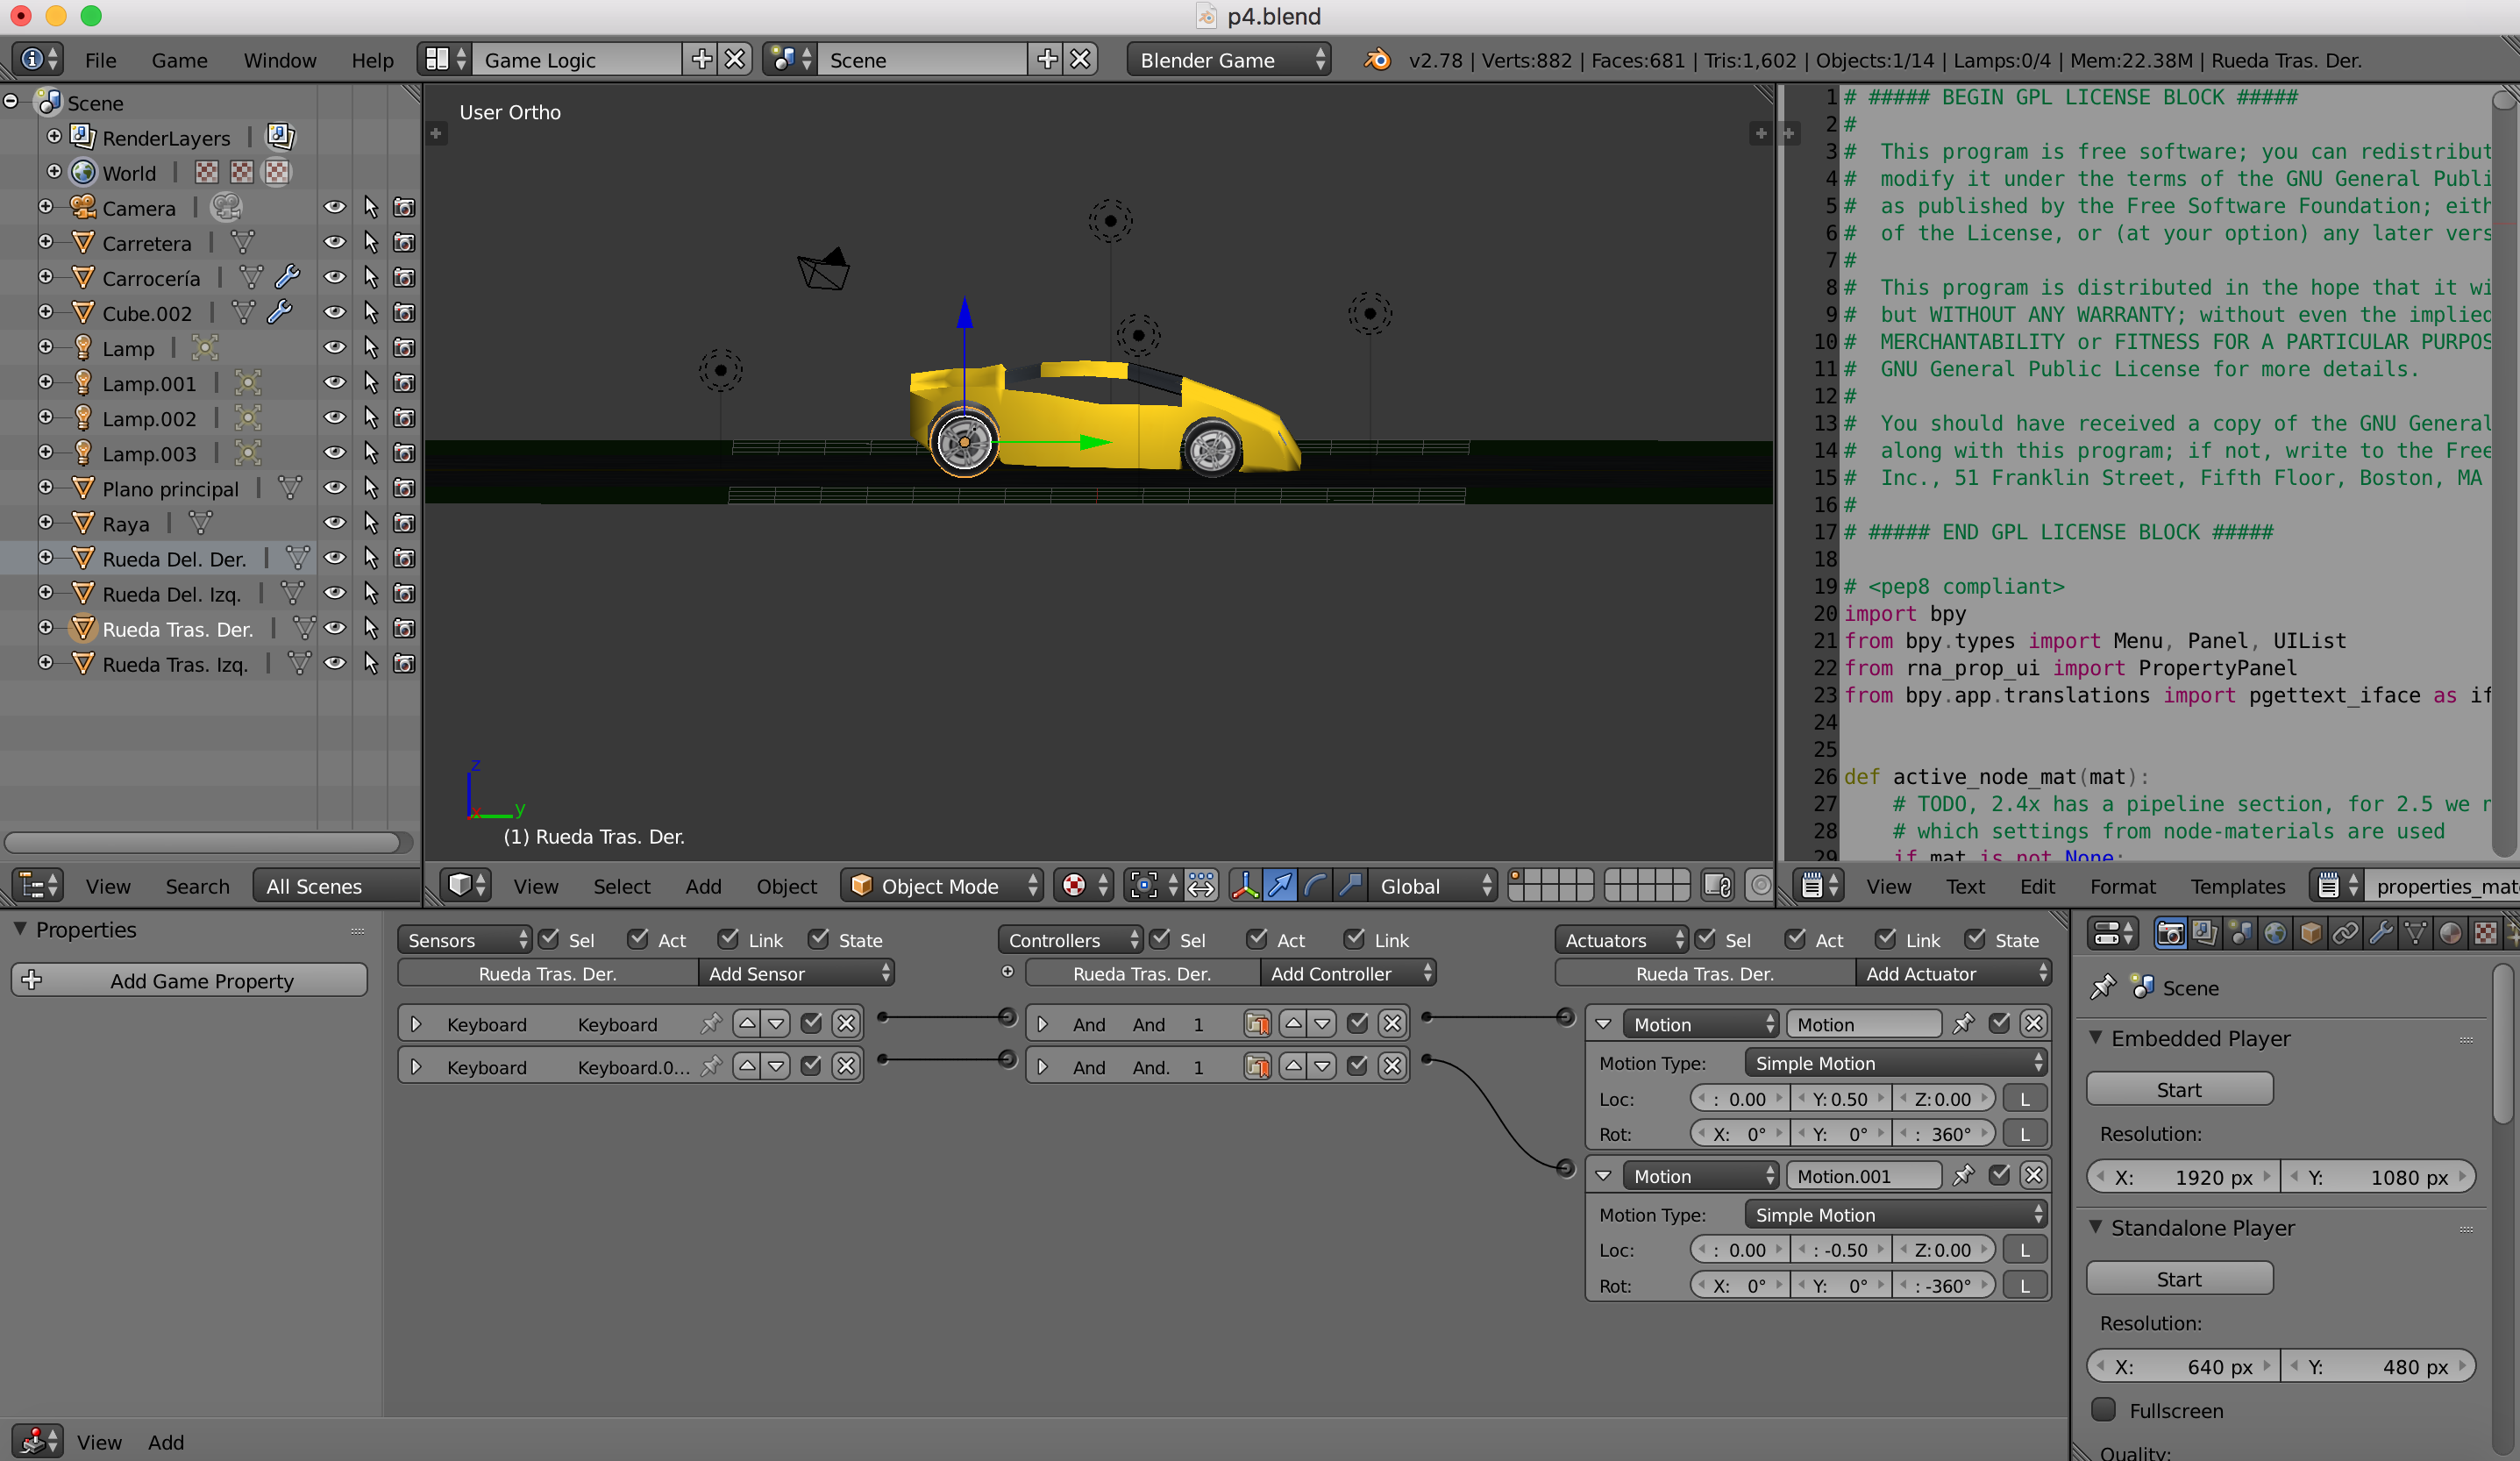
\includegraphics[width = 1.00\textwidth]{Imagenes/p4-img16}
 		\captionof{figure}{\label{fig:IPN}Configurando la vista de la cámara .} 
	\end{center} 
\end{figure}

\begin{figure}[H]
	\begin{center}
	 		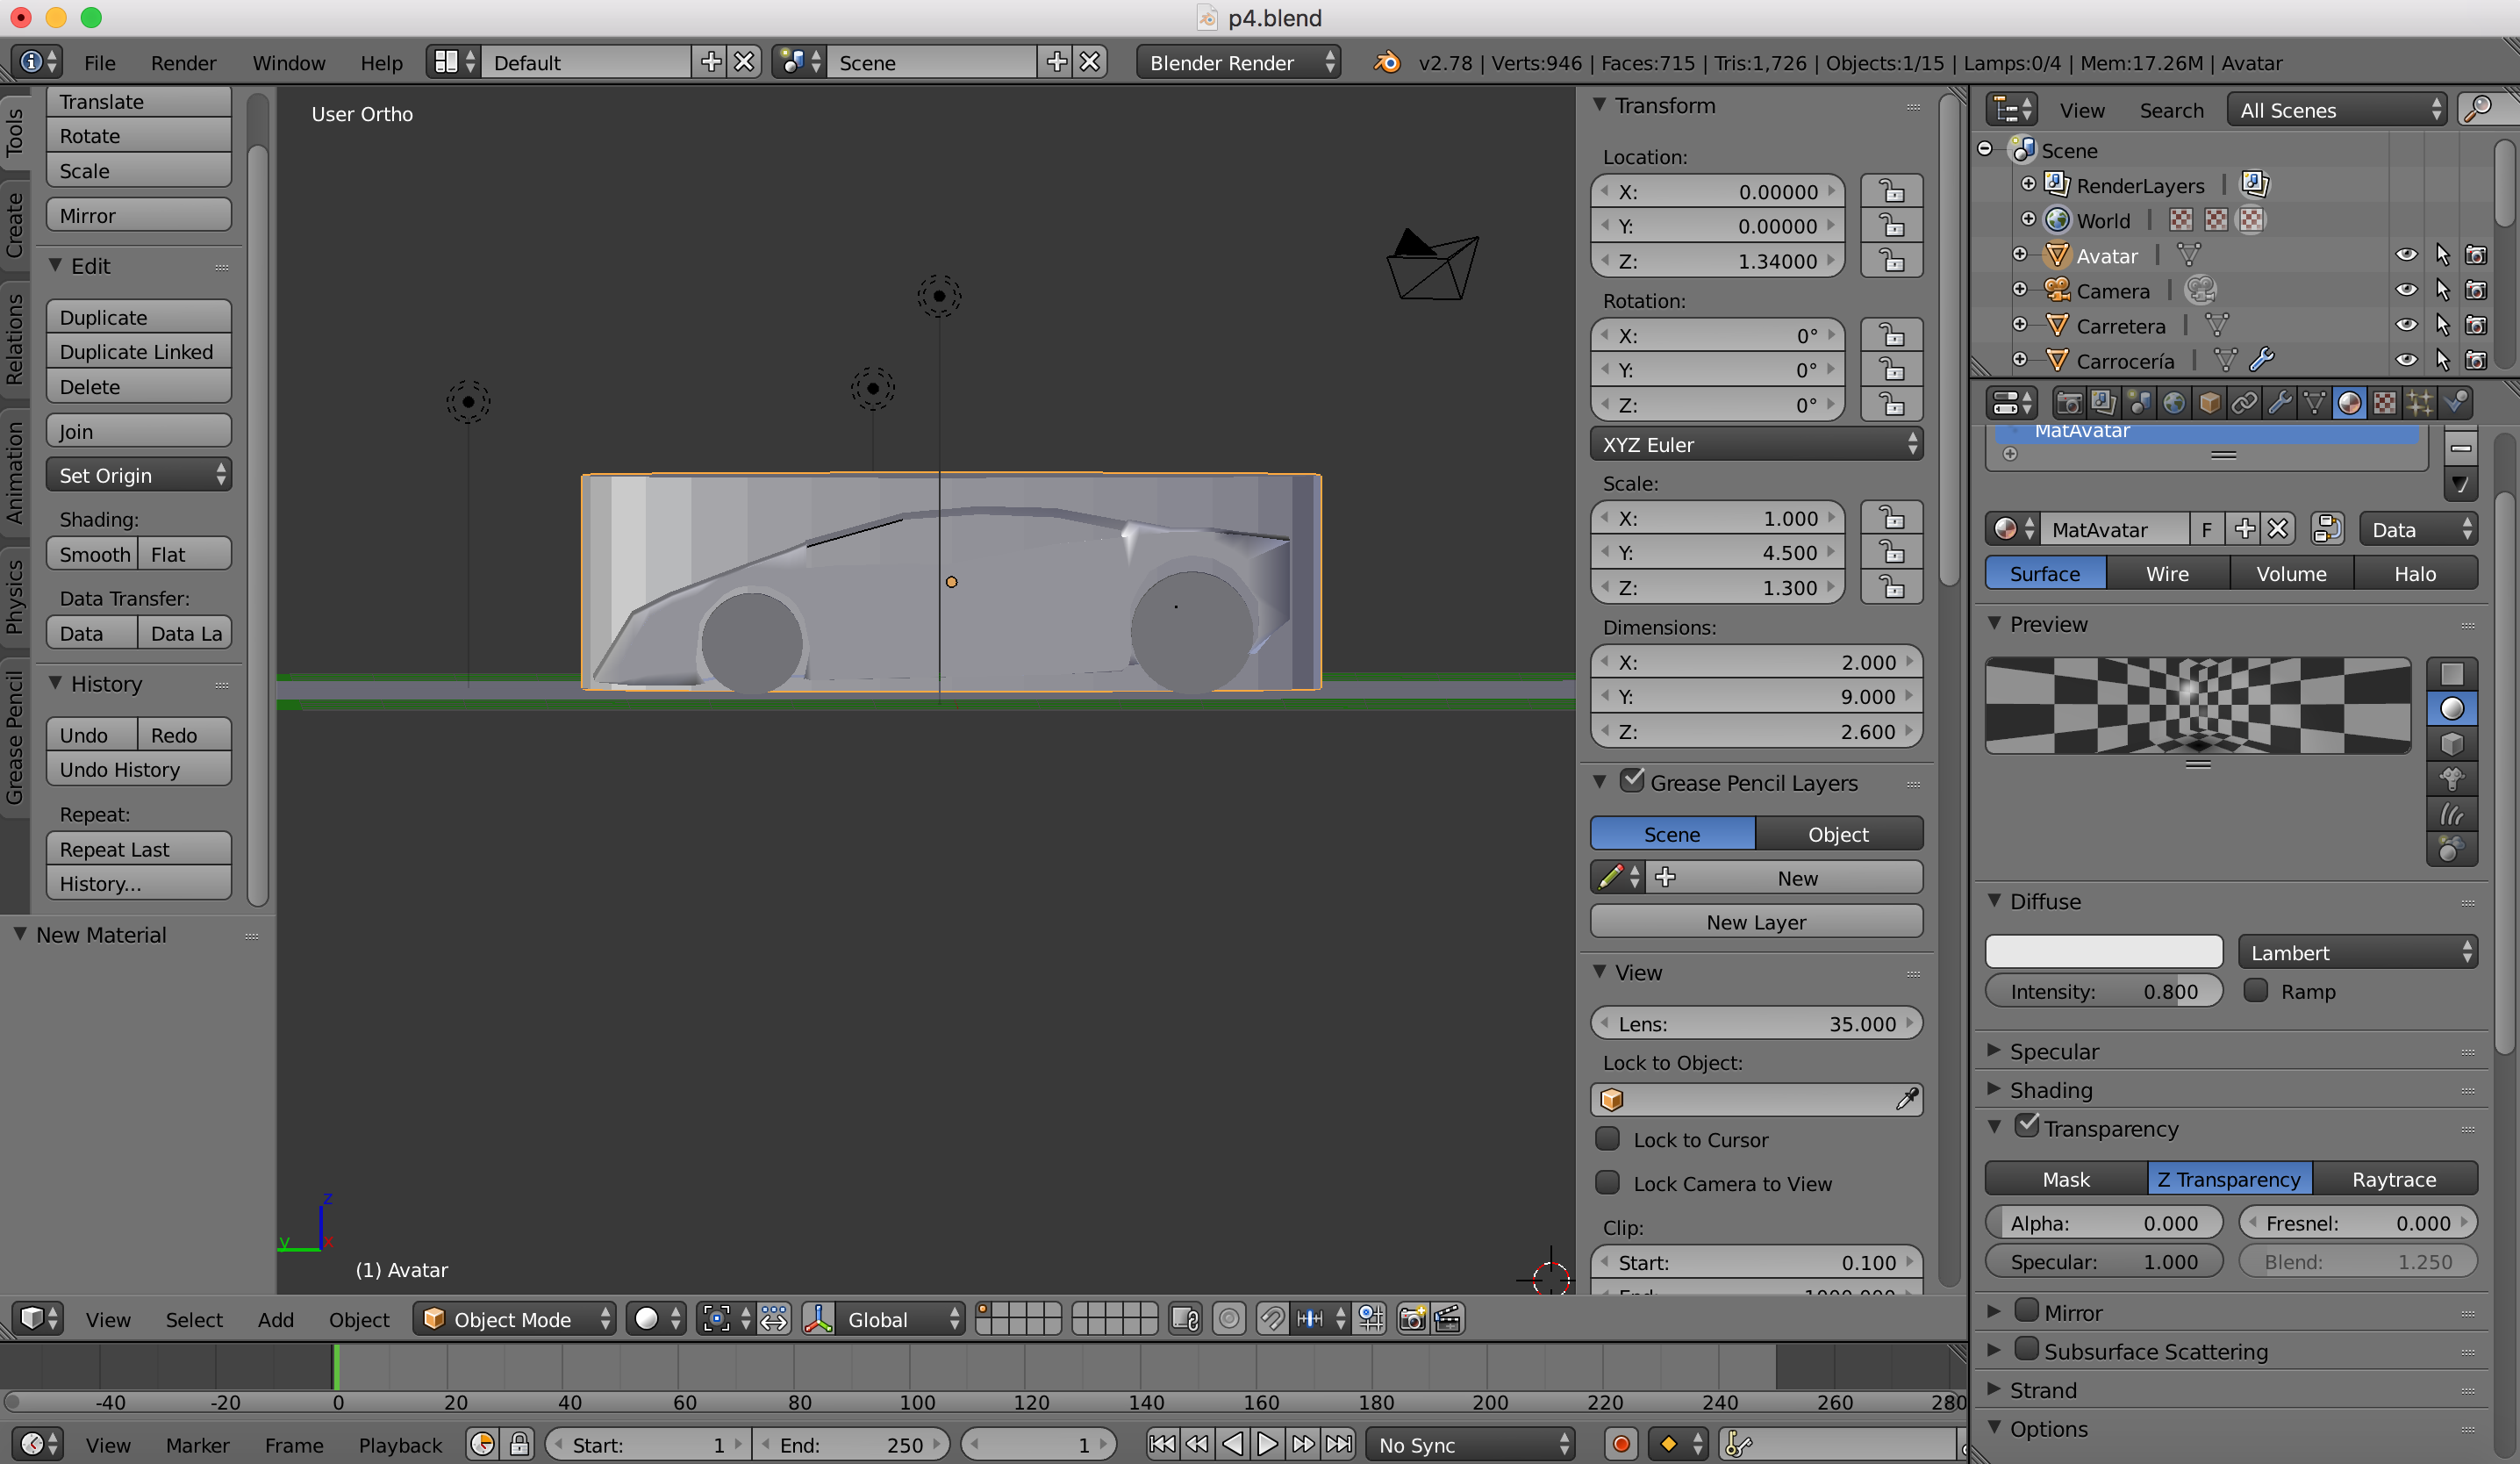
\includegraphics[width = 1.00\textwidth]{Imagenes/p4-img17}
 		\captionof{figure}{\label{fig:IPN}Ejecutando la interacción.} 
	\end{center} 
\end{figure}

En el documento zip referente a la entrega de la práctica se encuentral fichero de blender correspondiente a la misma y la memoria donde se detallan los pasos realizados.

\end{document}